%%%%%%%%%%%%%%%%%%%%%%%%%%%%%%%%%%%%%%%%%%%%%%%%%%%%%%%%%%%%%%%%%%%%%%%%%%%%%%%%%%%%%%%%%%%%%%%%%%%%%%%%%%%%%%%%%%%%%%%%%%%%%%%%%%%%%%%%%%%%%%%%%%%%%%%%%%%%%%%%%%%%%%%%%%%%%%%%%%%%
\chapter{Motivation}
\label{sec:Motivation}
Supersymmetry is able to offer solutions to unexplained phenomena in astrophysics and can solve the shortcomings of the Standard Model of particle physics (see Section~\ref{FIXME}).
Unfortunately, due to the unknown mechanism of supersymmetry breaking, the most general parametrisation of Supersymmetry introduces over 100 new parameters and thus opens up an incredibly large phenomenological space, 
leading to very different possible signatures at particle colliders. 
A variety of searches were hunting for SUSY during the Phase\,I run at the LHC in 2012.
Proton-proton collision data from the CMS and ATLAS experiments were analysed with a strong focus on the search for SUSY in the strong production sector (e.g. \cite{bib:CMS:RA2_8TeV,bib:CMS:MT2_8TeV,bib:ATLAS:JetPlusMET_8TeV}).
As a consequence, wide regions of SUSY parameter space are already excluded and 
the search for SUSY in more "exotic" regions gains more and more attention. 
Typical SUSY scenarios that are not easily excluded by the general SUSY searches consist of so-called compressed spectra where two or more particles are nearly mass-degenerate.
Such scenarios can have two very distinctive phenomenological properties.
First, if mother and daughter particles in a two body decay are almost mass-degenerate, the remaining decay product can be very soft in \pt, making them very hard to detect.
Second, the mother particle can be long-lived due to phase space suppression (see Section~\ref{sec:FIXME.Theory:Lifetimes}).
Because of these two properties, scenarios with compressed spectra can be challenging to search for and are in general much weaker constrained.\\

In R-parity conserving Supersymmetry, compressed spectra can be realised if the lightest neutralino ($\chi^{0}_1$) is almost mass-degenerate with the lightest chargino ($\chi^{\pm}_1$).
Such a mass-degeneracy naturally occurs in case of wino-like neutralinos and charginos, since the mass gap between $W_{3}$ and $W_{1/2}$ is fully determined by higher loop corrections (see Section~\ref{FIXME}).
SUSY models with a wino-like lightest neutralino are especially interesting because they are able to explain the sources of the relic density FIXME \cite{}. 
While it is not possible to explain the full relic density with thermally produced neutralinos for m$_{\chi^{0}_1}\lesssim 2.9\,\tev$ \cite{bib:Ibe:DarkMatter_2015}, neutralinos can still be the dominant part if they are non-thermally produced via the decay of a long-lived particle such as a wino-like chargino \cite{bib:Moroi:DarkMatter_2013}.\\

%Additionaly, due to the large annihilation cross-sections for a wino-like neutralino \cite{bib:Hisano:DarkMatter_2003}, these models would result in strong signals in indirect searches.\\

At the LHC, there are several possible chargino production channels. 
Chargino pairs can be produced through a photon or a $Z$-boson exchange. 
The chargino then decays via a virtual $W$-boson to the lightest neutralino and a fermion pair (e.g. a pion). 
This process is illustrated in the Feynman diagram in Fig.~\ref{fig:FeynmanDiagram}.


Other possible chargino pair production channels include the exchange of a supersymmetric Higgs boson or a t-channel squark exchange (Fig.~\ref{fig:FeynmanDiagramProductionCharginoPair}).


Apart from pair production, charginos can be produced via the chargino neutralino production channel. 
On tree-level, there exist two production mechanisms: the s-channel $W$-boson exchange and the t-channel squark exchange (Fig.~\ref{fig:FeynmanDiagramProductionCharginoNeutralino}).
\begin{figure}[!h]
  \centering 
  \begin{tabular}{c}
    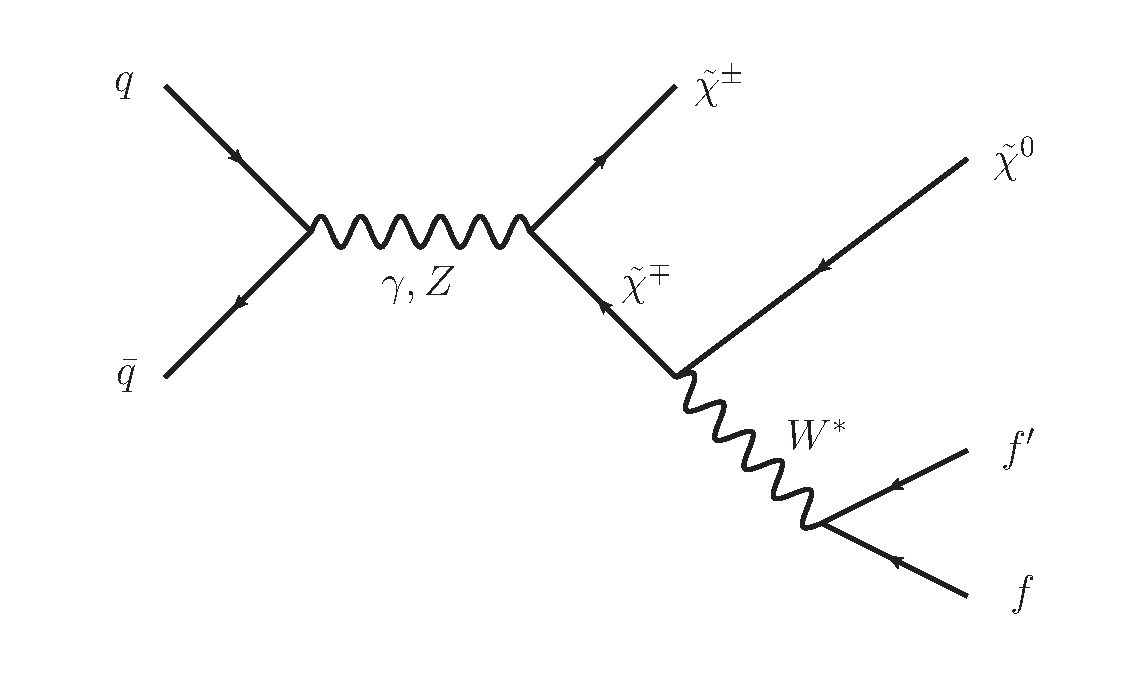
\includegraphics[width=0.75\textwidth]{figures/analysis/ChiChi_ProductionAndDecay.pdf}
  \end{tabular}
  \caption{Feynman diagram of chargino pair production via gamma or $Z$-boson exchange and the subsequent decay via a virtual $W$-boson.}
  \vspace{30pt}
  \label{fig:FeynmanDiagram}
\end{figure}

\begin{figure}[!h]
  \centering 
  \begin{tabular}{c}
    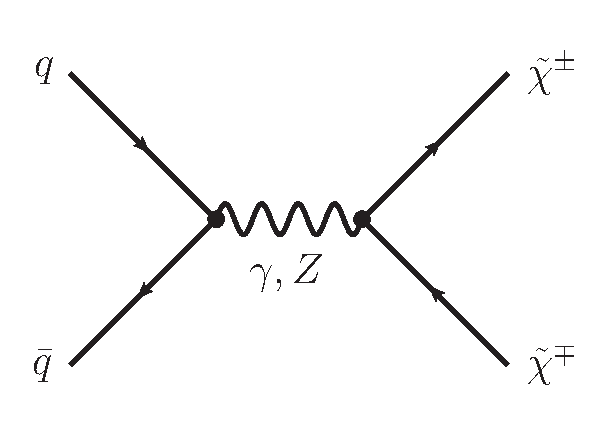
\includegraphics[width=0.33\textwidth]{figures/analysis/ChiChi_GammaZ.pdf}
    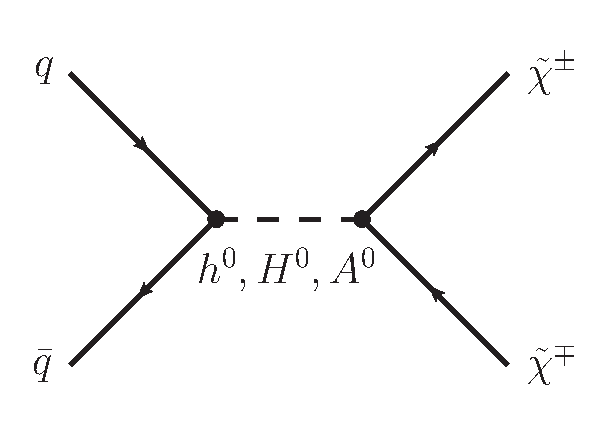
\includegraphics[width=0.33\textwidth]{figures/analysis/ChiChi_Scalar.pdf}
    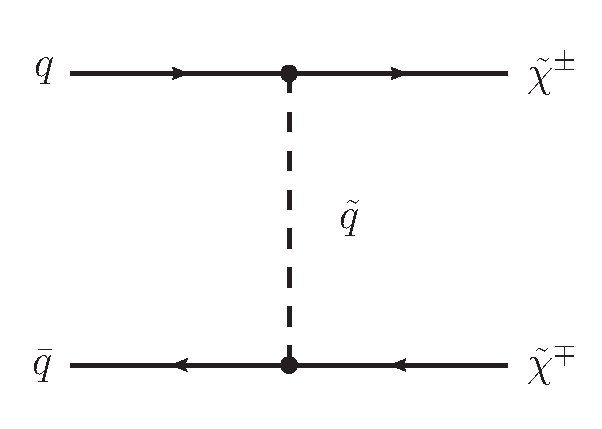
\includegraphics[width=0.33\textwidth]{figures/analysis/ChiChi_Squark.pdf}
  \end{tabular}
  \caption{Main tree-level diagrams for chargino pair production.}
   \vspace{30pt}
  \label{fig:FeynmanDiagramProductionCharginoPair}
\end{figure}

\begin{figure}[!h]
  \centering 
  \begin{tabular}{c}
    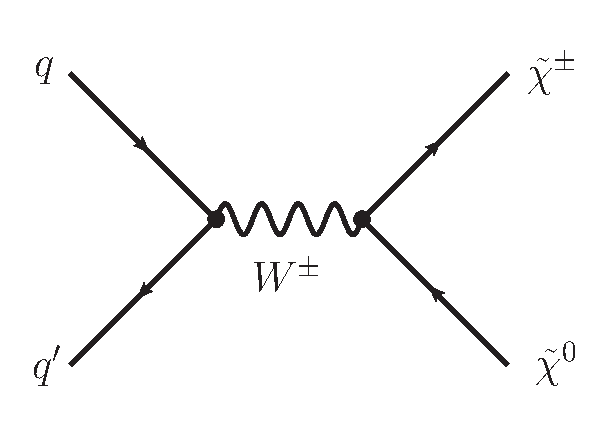
\includegraphics[width=0.33\textwidth]{figures/analysis/ChiChi0_WBoson.pdf}
    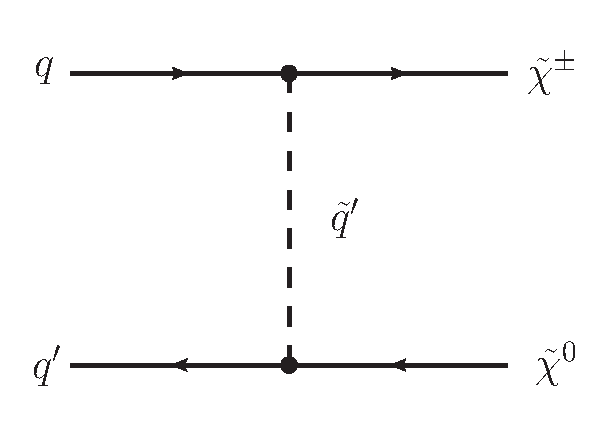
\includegraphics[width=0.33\textwidth]{figures/analysis/ChiChi0_Squark.pdf}
  \end{tabular}
  \caption{Main tree-level diagrams for chargino neutralino production.}
  \label{fig:FeynmanDiagramProductionCharginoNeutralino}
\end{figure}
Thus, the LHC offers the potential to search for charginos and due to its high centre-of-mass energy it is the first collider that can access SUSY models with charginos of several hundreds \gev.

%Thus, the LHC offers the potential to search for charginos and is therefore well suited to %investigate SUSY models with long-lived charginos. FIXME: is lhc the only machine that can %produce charginos?

Although supersymmetric models with nearly mass-degenerate \chipm and \chiO lead to exotic signatures with long lived charginos and soft decay products, existing SUSY searches at CMS can in principle be sensitive to these models. The exclusion power of existing SUSY searches can be assessed by interpreting their results in terms of the fraction of excluded parameter points in the phenomenological MSSM (see Section~\ref{theorySUSY} for a detailed introduction to the pMSSM). The results of such a study which has been performed in \cite{bib:CMS:DT_8TeV} are shown in Figure~\ref{fig:pMSSMplot}. 
\begin{figure}[!t]
  \centering 
  \begin{tabular}{c}
    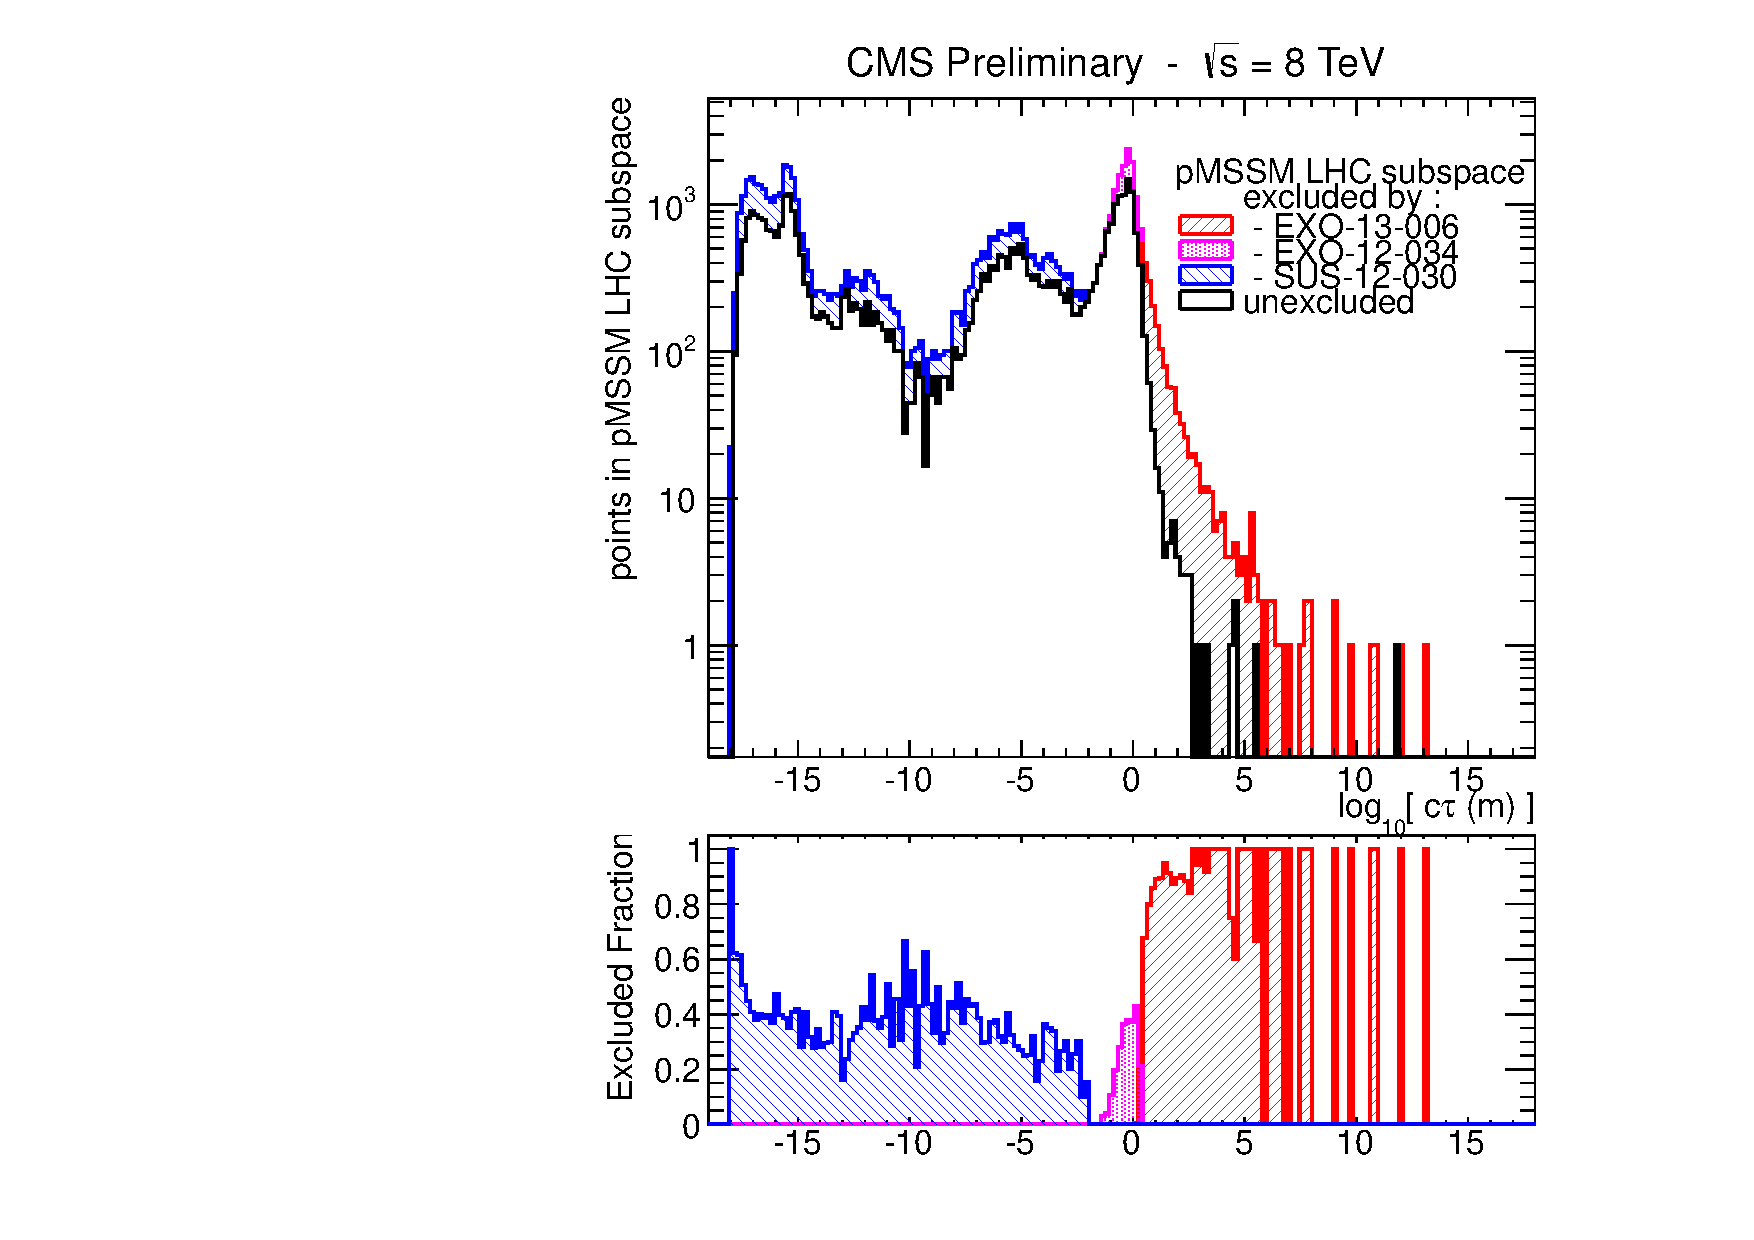
\includegraphics[width=0.75\textwidth]{figures/analysis/pMSSM_vs_ctau.pdf}
  \end{tabular}
  \caption{The number of excluded pMSSM points at 95\% C.L. (upper part) and the fraction of excluded pMSSM points (bottom part) vs. the chargino lifetime for different CMS searches.
           Red area: the search for long-lived charged particles \cite{bib:CMS:HSCP_8TeV},
           Purple area: the search for disappearing tracks  \cite{bib:CMS:DT_8TeV},
           Blue area: a collection of various general SUSY searches \cite{bib:CMS:pMSSMinterpretation_7TeV_PAS}
           The black line indicates the unexcluded pMSSM parameter points.
           The sampling of the parameter space points was done according to a prior probability density function which takes pre-LHC data and results from indirect SUSY searches into account (see \cite{bib:CMS:HSCPReinterpreation_PAS} for further details).
           Taken from: \cite{bib:pMSSMplot_source_from_DT}.}
  \label{fig:pMSSMplot}
\end{figure}
It can be seen that general SUSY searches (blue area) are mostly sensitive to shorter chargino lifetimes ($c\tau \lesssim 10\cm$)\footnote{It should be mentioned, that the pMSSM interpretation relied on the use of fast simulation techniques which are not capable of simulating charginos with lifetimes $\ctau>1\cm$. It could therefore not be tested to which exact upper lifetime the searches combined in the blue area are sensitive to.}.. 
Two existing searches, the search for long-lived charged particles~\cite{bib:CMS:HSCP_8TeV} and the search for disappearing tracks~\cite{bib:CMS:DT_8TeV} focus on long and intermediate chargino lifetimes respectively. 
These two searches (purple and red areas) are sensitive to chargino lifetimes of $\gtrsim 35\cm$. 
Taken together, the existing searches exclude a large fraction of pMSSM points at different chargino lifetimes. 
However, there is a gap between the general SUSY searches and the search for disappearing tracks where none of the existing searches show a high sensitivity.

The here presented analysis aims at targeting this gap by focusing on charginos with intermediate lifetimes of $10\cm \lesssim c\tau \lesssim 40\cm$. 
The main idea is to make use of the variable $dE/dx$ which can be very discriminating for massive particles such as charginos.
The associated challenges and the general strategy of this analysis will be presented in the next section.


%%%%%%%%%%%%%%%%%%%%%%%%%%%%%%%%%%%%%%%%%%%%%%%%%%%%%%%%%%%%%%%%%%%%%%%%%%%%%%%%%%%%%%%%%%%%%%%%%%%%%%%%%%%%%%%%%%%%%%%%%%%%%%%%%%%%%%%%%%%%%%%%%%%%%%%%%%%%%%%%%%%%%%%%%%%%%%%%%%%%
%%%%%%%%%%%%%%%%%%%%%%%%%%%%%%%%%%%%%%%%%%%%%%%%%%%%%%%%%%%%%%%%%%%%%%%%%%%%%%%%%%%%%%%%%%%%%%%%%%%%%%%%%%%%%%%%%%%%%%%%%%%%%%%%%%%%%%%%%%%%%%%%%%%%%%%%%%%%%%%%%%%%%%%%%%%%%%%%%%%%
\chapter{General search strategy}
\label{sec:GeneralSearchStrategy}

When searching for supersymmetric models with long-lived \chipm, the strategy is of course highly dependent on the actual lifetime of the chargino. 
For long lifetimes, the chargino can reach the muon chambers and can be reconstructed as a muon even despite a longer time-of-flight \cite{bib:CMS:HSCP_7TeV}. 
For lower lifetimes, the chargino can already decay inside the detector (e.g. the tracker), and can hence not be reconstructed as a muon but leads to an isolated, potentially disappearing track in the tracker. 
The detector signatures of these two scenarios are visualised in Fig.~\ref{fig:CharginoPaiEventDisplay}, where simulated chargino-chargino events are shown in a cross-sectional view of the CMS detector.
\begin{figure}[!b]
  \centering 
  \begin{tabular}{c}
  \begin{subfigure}{0.31\textwidth}
    \frame{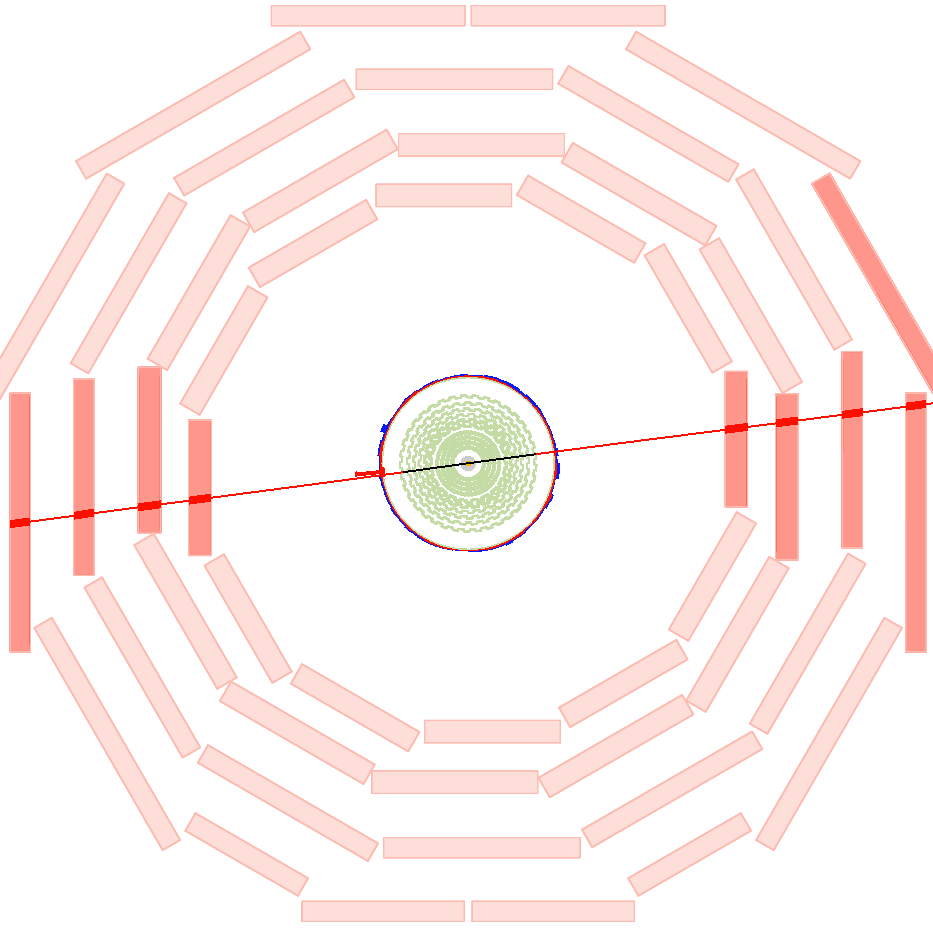
\includegraphics[width=0.99\textwidth]{figures/analysis/MotivationAndGeneralSearchStrategy/CharginoPairEvent_ctau_10000cm_lumi_1_event_12015.png}}
      \caption{}
  \end{subfigure} 
  \begin{subfigure}{0.31\textwidth}
    \frame{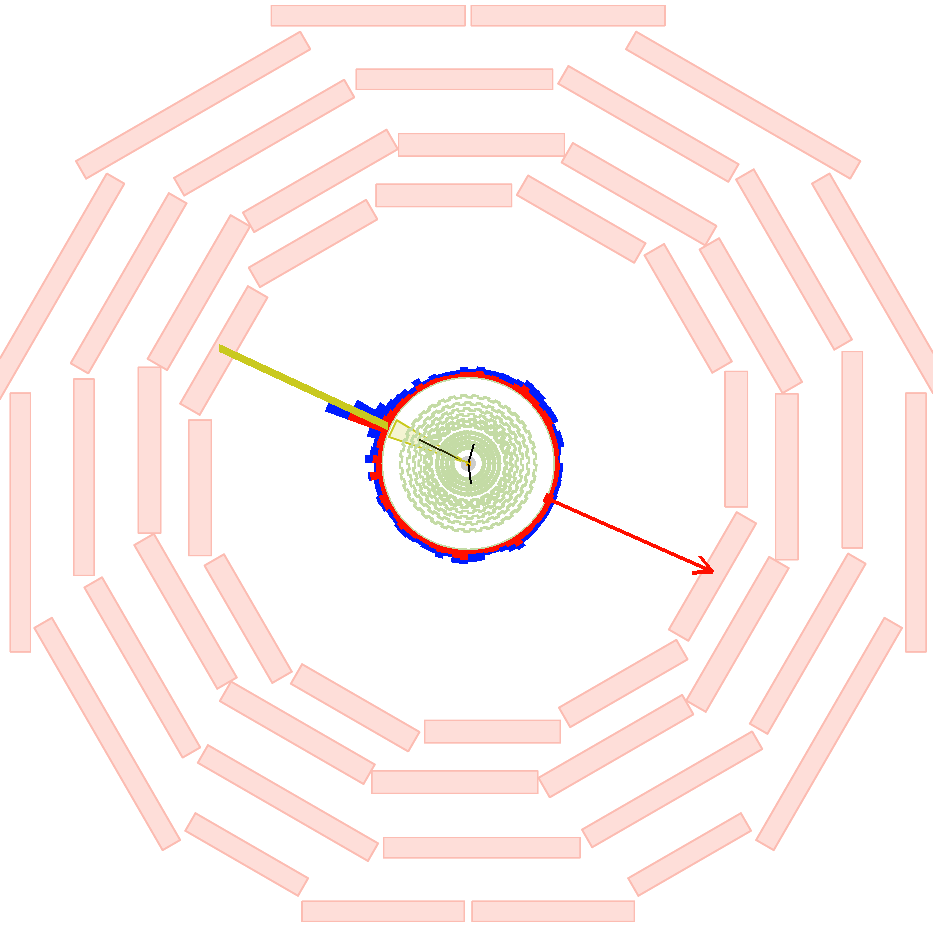
\includegraphics[width=0.99\textwidth]{figures/analysis/MotivationAndGeneralSearchStrategy/CharginoPairEvent_ctau_50cm_lumi_1_event_11024.png}}
      \caption{}
  \end{subfigure} 
  \begin{subfigure}{0.31\textwidth}
      \frame{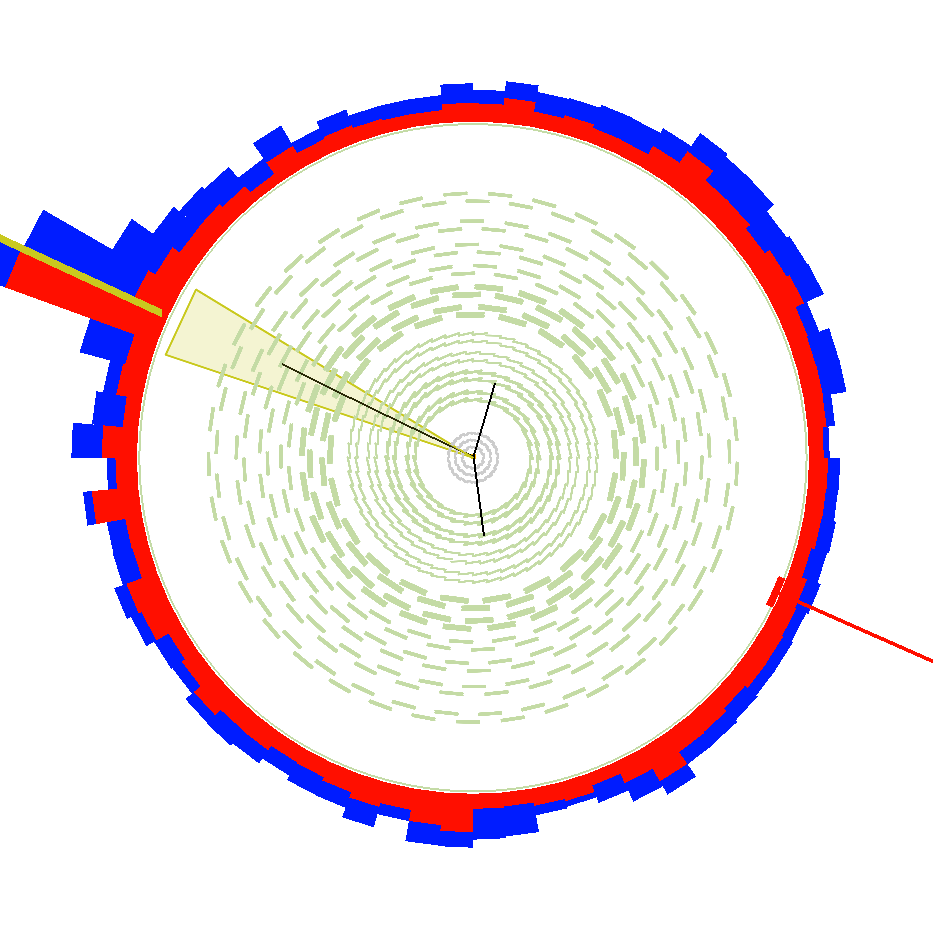
\includegraphics[width=0.99\textwidth]{figures/analysis/MotivationAndGeneralSearchStrategy/CharginoPairEvent_ctau_50cm_lumi_1_event_11024_Zoom.png}}
      \caption{}
  \end{subfigure} 
  \end{tabular}
  \caption{Visualisation of possible signatures of a chargino pair produced with a lifetime of $c\tau = 10\,\text{m}$ (a) and a lifetime of $c\tau = 0.5\,\text{m}$ (b and c). 
           In the left picture, both charginos are reconstructed as muons, which can be seen in the energy deposition in the muon chambers (red boxes). 
           In the middle picture both charginos are only visible as tracks in the tracker (black lines), where both trajectories end inside the silicon strip tracker, showing the decay point of the corresponding chargino. 
           The right picture is a zoom of the picture in the middle. Here, only the cross-section of the tracker (green wavy lines for the strip and grey lines for the pixel) is displayed. The red arrow shows the missing transverse energy in the event.
           The red (blue) towers correspond to the energy deposition in the ECAL (HCAL).} 
  \label{fig:CharginoPaiEventDisplay}
\vspace{10pt}
\end{figure}

Since this analysis targets a search for Supersymmetry with charginos of lifetimes between $10\,\text{cm} \lesssim c\tau \lesssim  40\,\text{cm}$, the charginos decay rather early in the detector, even in the inner layers of the tracker. 
Thus, the signature of the chargino consists of an isolated track and the signatures of the decay products, i.e. of a neutralino and a fermion pair. 
In case of R-parity conservation the neutralino is stable and weakly interacting, thus traversing the detector without leaving any further signature.
The missing transverse energy of the neutralino is balanced by the missing transverse energy of the second produced SUSY particle.
This is either a neutralino or the decay products of the chargino in events with chargino pairs. 

The signature of the fermion pair can in principle be used to select chargino events. 
However, for mass-degenerate charginos, it can be very hard or even impossible to detect these fermions as will be explained in detail in the next paragraph.

First of all, the fermionic decay product (e.g. a pion) can hardly be reconstructed because it does not origin from the primary vertex.
Secondly, it is very low in momentum because of the mass-degeneracy between \chipm and \chiO.
The typical momentum of a pion originating from a chargino to neutralino decay in the \chipm rest frame is of the order 
\begin{equation*}
p_{\pi}\sim \sqrt{m_{\chi^{\pm}_1}-m_{\chi^{0}_1}-m_{\pi}}.
\end{equation*}
%As the \chipm is rather slow for higher masses this is a good approximation also in the detector rest frame.
For a mass gap between \chipm and \chiO of $\Delta m=150\, \mev$, the pt distribution of the resulting pion peaks \mbox{at $\sim$ 100\,\mev} and ends at \mbox{\pt $\sim 400\,$\mev} (Fig.~\ref{fig:KinkedTrack}).

\begin{figure}[!b]
  \centering 
  \begin{tabular}{c}
    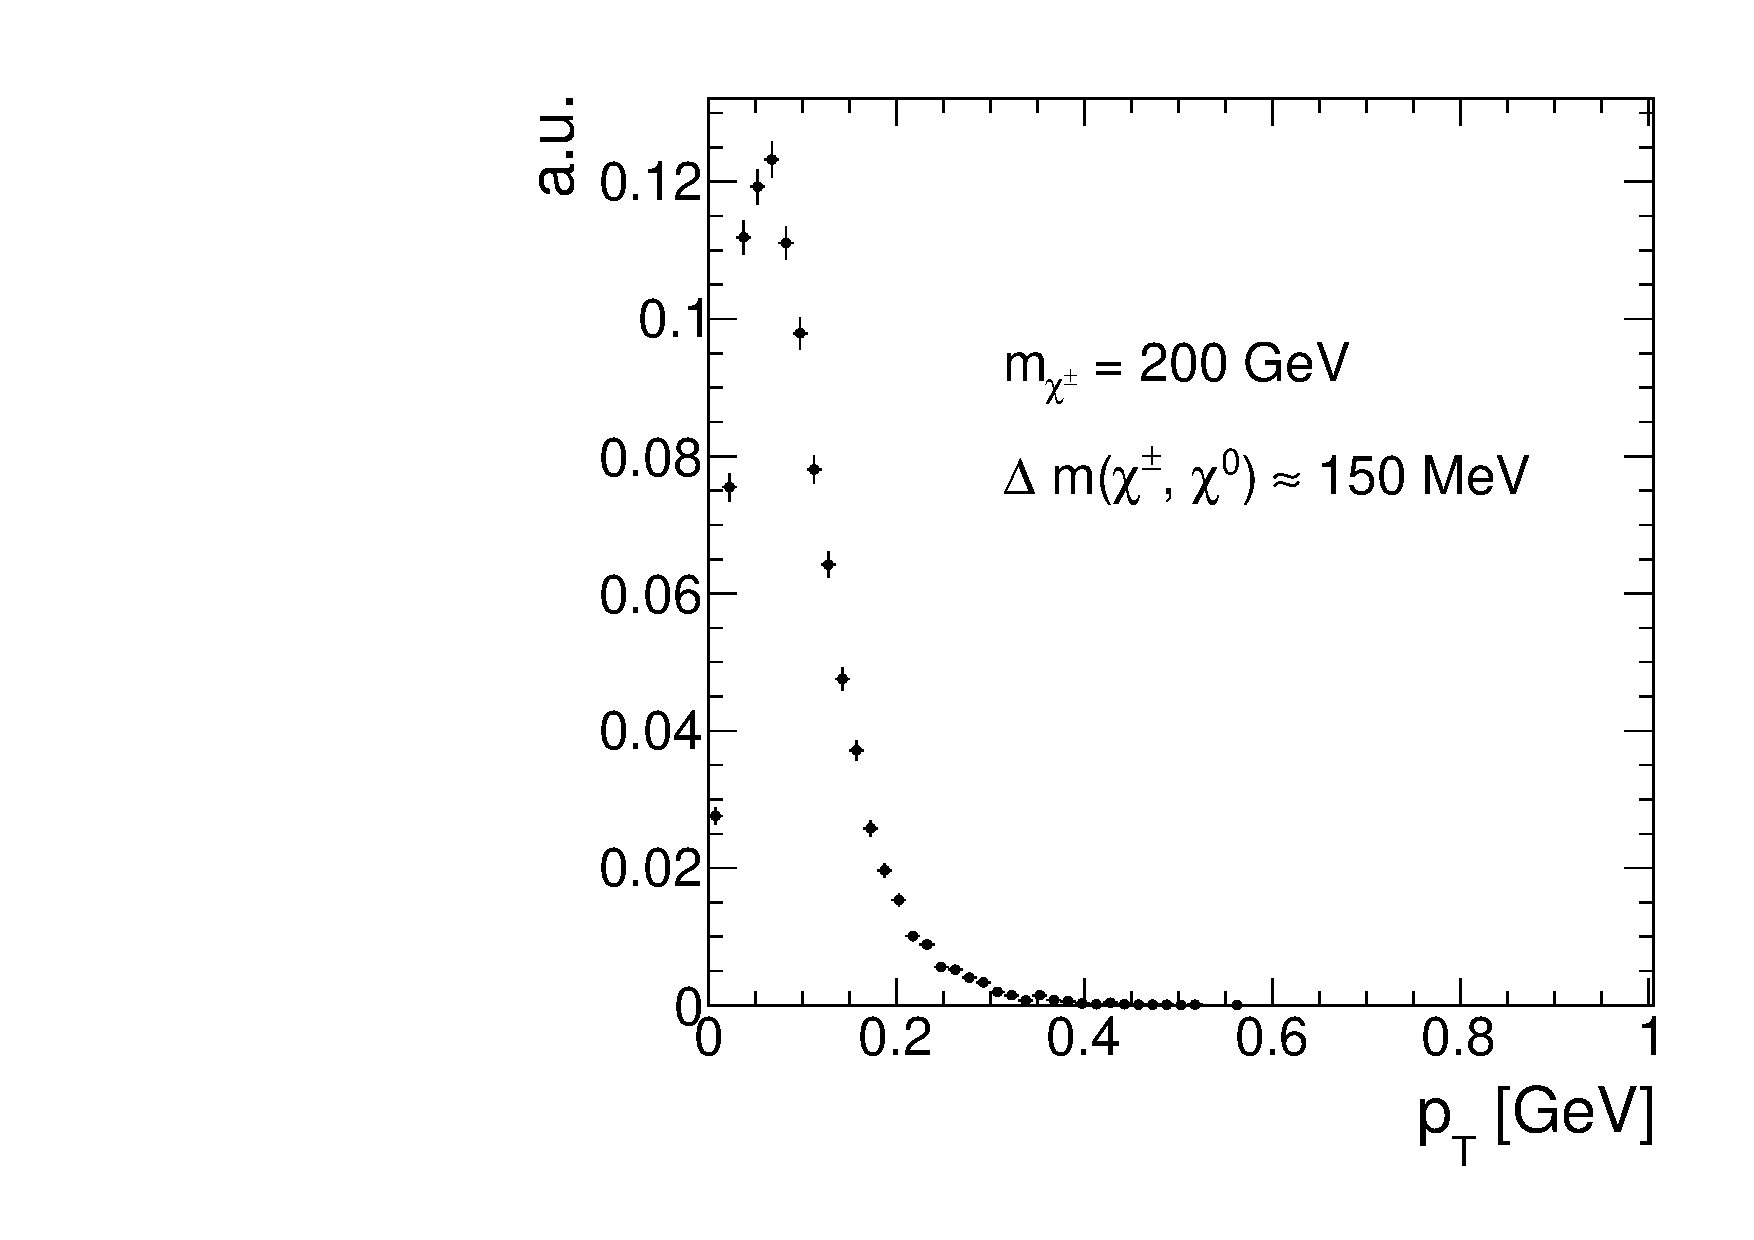
\includegraphics[width=0.49\textwidth]{figures/analysis/PtOfPions.pdf}
  \end{tabular}
  \caption{Transverse momentum distribution of pions coming from chargino decay into a neutralino with a mass gap of 150\mev.}
  \label{fig:ptOfPions}
\end{figure} 

If the transverse momentum of a particle is very low, the particle trajectory is much more bended compared to a particle with higher \pt (see Fig.~\ref{fig:KinkedTrack} for illustration).
\begin{figure}[!b]
  \centering 
  \begin{tabular}{c}
    \frame{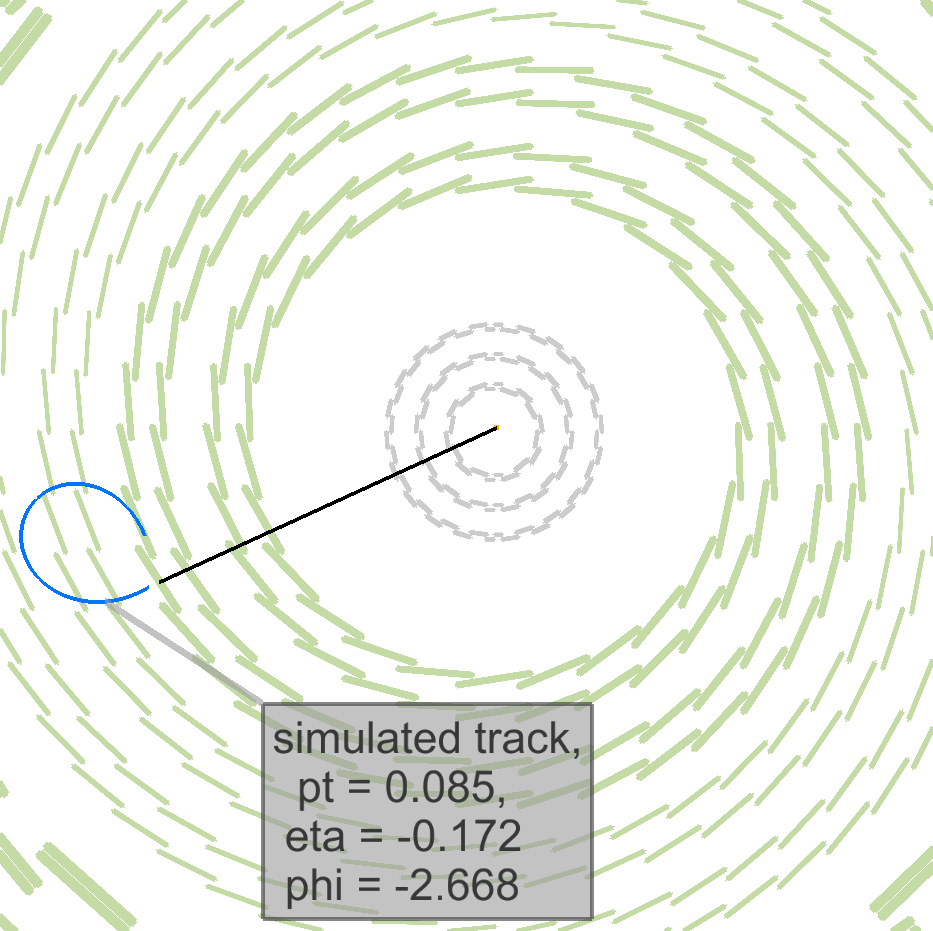
\includegraphics[width=0.30\textwidth]{figures/analysis/MotivationAndGeneralSearchStrategy/BendedPionTrack.png}}
    %\frame{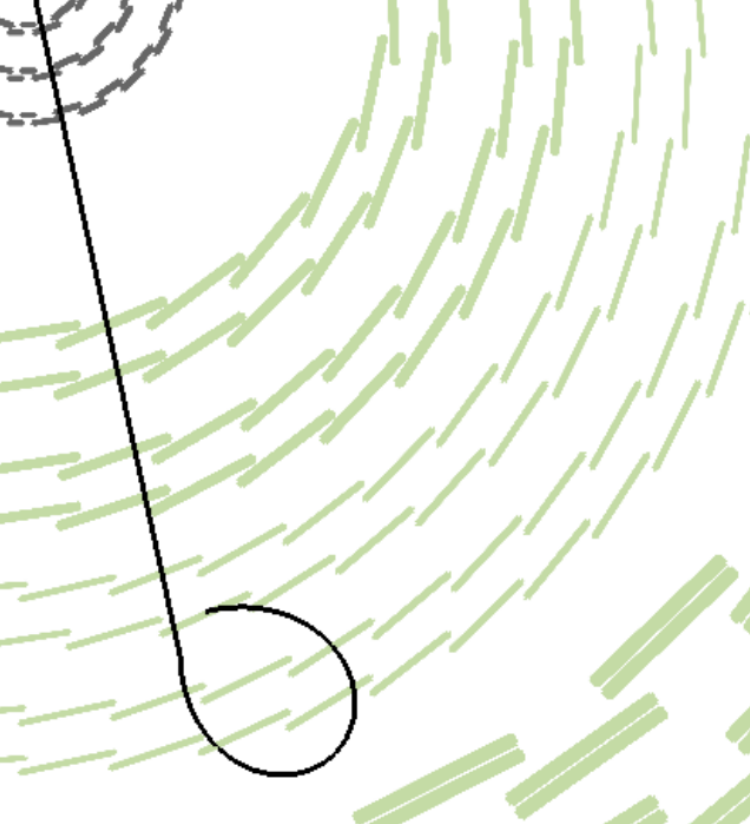
\includegraphics[width=0.30\textwidth]{figures/analysis/KinkedTrackZoom_Quadrat.png}}
  \end{tabular}
  \caption{Cross-sectional view of the tracker (silicon strip (silicon pixel) tracker layers are illustrated with green (grey) lines) and a simulated chargino track (black line) decaying to a pion (bended blue line) with a \pt of $\sim$85\mev and a neutralino (not visible).}
  \label{fig:KinkedTrack}
\end{figure} 
Due to this bending, the track reconstruction efficiency of particles with a transverse momentum below 1\gev decreases rapidly, reaching around 40\% for isolated pions with a \pt of 100\mev~\cite{bib:CMS:tracking_8TeV}. 
It is therefore impossible to rely on a reconstruction of the fermionic chargino decay products in this analysis.

In summary, the signature of chargino events in mass-degenerate SUSY models consists only of a – potentially disappearing- track. 
Such a signature is very difficult to detect, especially since CMS doesn't offer a dedicated track trigger so that triggering on the chargino track is impossible.

In order to search for such signatures, one therefore needs to trigger on other, less obvious properties of chargino events. 
This analysis takes advantage of higher order contributions to the Feynman diagrams shown in the previous sections (Figs.~\ref{fig:FeynmanDiagramProductionCharginoPair}, \ref{fig:FeynmanDiagramProductionCharginoNeutralino}), resulting in initial state radiation (ISR).
If the initial quarks radiate a high \pt gluon, the resulting jet can be detected and can offer a possibility to search for events with nothing more than isolated tracks.
Furthermore, the non-detection of the chargino's decay products plus a high \pt ISR jet lead to missing transverse energy (MET) in the event. 
Exploiting these two circumstances, it is possible to detect chargino-pair or chargino-neutralino events with the help of Jet+MET triggers.

Since Jet+MET triggers are not very specific for chargino events, it is important to identify further track properties that can be used to select chargino candidates.
One distinctive property of charginos compared to SM particles is their high mass. 
Therefore, charginos can be identified by selecting high \pt tracks. 
Furthermore, the energy loss per path length ($dE/dx$) depends quadratically on the particle's mass for low velocities ($0.2<\beta\gamma<0.9$):
\begin{equation*}
\langle\frac{dE}{dx}\rangle = K \frac{m^2}{p^2} +C
\end{equation*}
Therefore, $dE/dx$ constitutes a very nice discriminating variable for massive particles like charginos against SM particles.
The selection of chargino events in this analysis thus relies on the selection of isolated high \pt tracks with high $dE/dx$ values. 

If the chargino decays before it has crossed the full pixel and strip detector, the associated track is disappearing. 
For low lifetimes, the tracks can be very short and can have only a few hits in the detector. 
In order to reconstruct a particle's trajectory, a minimum of three hits are required since defining a helical path requires five parameters (see \cite{bib:CMS:tracking_8TeV}). 
A specific challenge for this analysis is hence the combination of searching for short tracks and utilising the measurement of the energy deposition of the chargino. 
For very short tracks, eventually only passing the first couple of layers of the whole tracker system, the pixel tracker information becomes very important. 
Therefore, an accurate energy measurement in the pixel system is of great importance to this analysis. 
However, no other CMS analysis has used the energy information of the pixel tracker so far.
This analysis thus requires a thorough study of the quality of the pixel energy calibration and, potentially, a recalibration in case the pixel energy calibration is not sufficient.



\section{Comparison to existing searches}
As already mentioned before, there are several analyses at CMS at $\sqrt{s}=8\,\tev$ with 20\,fb$^{-1}$ data, that are sensitive to intermediate lifetime charginos, most notably the search for long-lived charged \mbox{particles \cite{bib:CMS:HSCP_8TeV}} and the search for disappearing tracks \cite{bib:CMS:DT_8TeV}.
The here presented analysis aims at achieving an increase in sensitivity towards shorter lifetimes compared to the existing analyses in a twofold way.
First, the selection is optimised for the inclusion of very short tracks.
Second, the inclusion of the variable $dE/dx$ is used to increase the search sensitivity compared to \cite{bib:CMS:DT_8TeV}.\\

In \cite{bib:CMS:HSCP_8TeV}, a minimum number of eight hits were required for every track, whereas \cite{bib:CMS:DT_8TeV} required a minimum of seven hits.
This can be very inefficient for shorter lifetimes, where most of the charginos already decay shortly after the pixel tracker.
In Fig.~\ref{fig:NHits_2Signal_noSelection_normalized} (left), the normalised distribution of the number of measurements (\nhits) of chargino tracks is shown. 
It can be seen, that \nhits peaks at the minimal possible value needed for track reconstruction of $\nhits=3$ for lower lifetimes.
For higher lifetimes ($\ctau=50\cm$) the distribution shifts to higher values with a second peak at $\nhits\sim17$.
However, a notable fraction of $\sim$ 40\% of chargino tracks still has a number of measurements of $\nhits<8$. 

It should be also mentioned, that the track reconstruction efficiency is sufficient for short chargino tracks, such that a loosening of the \nhits requirement is expected to be really improving the signal acceptance.
The track reconstruction efficiency for different chargino decay points is depicted in Fig.~\ref{fig:NHits_2Signal_noSelection_normalized} (right).
For very short tracks ($\nhits=3$) the efficiency is still around 20\%.\\
\begin{figure}[!bt]
  \centering 
  \begin{tabular}{c}
  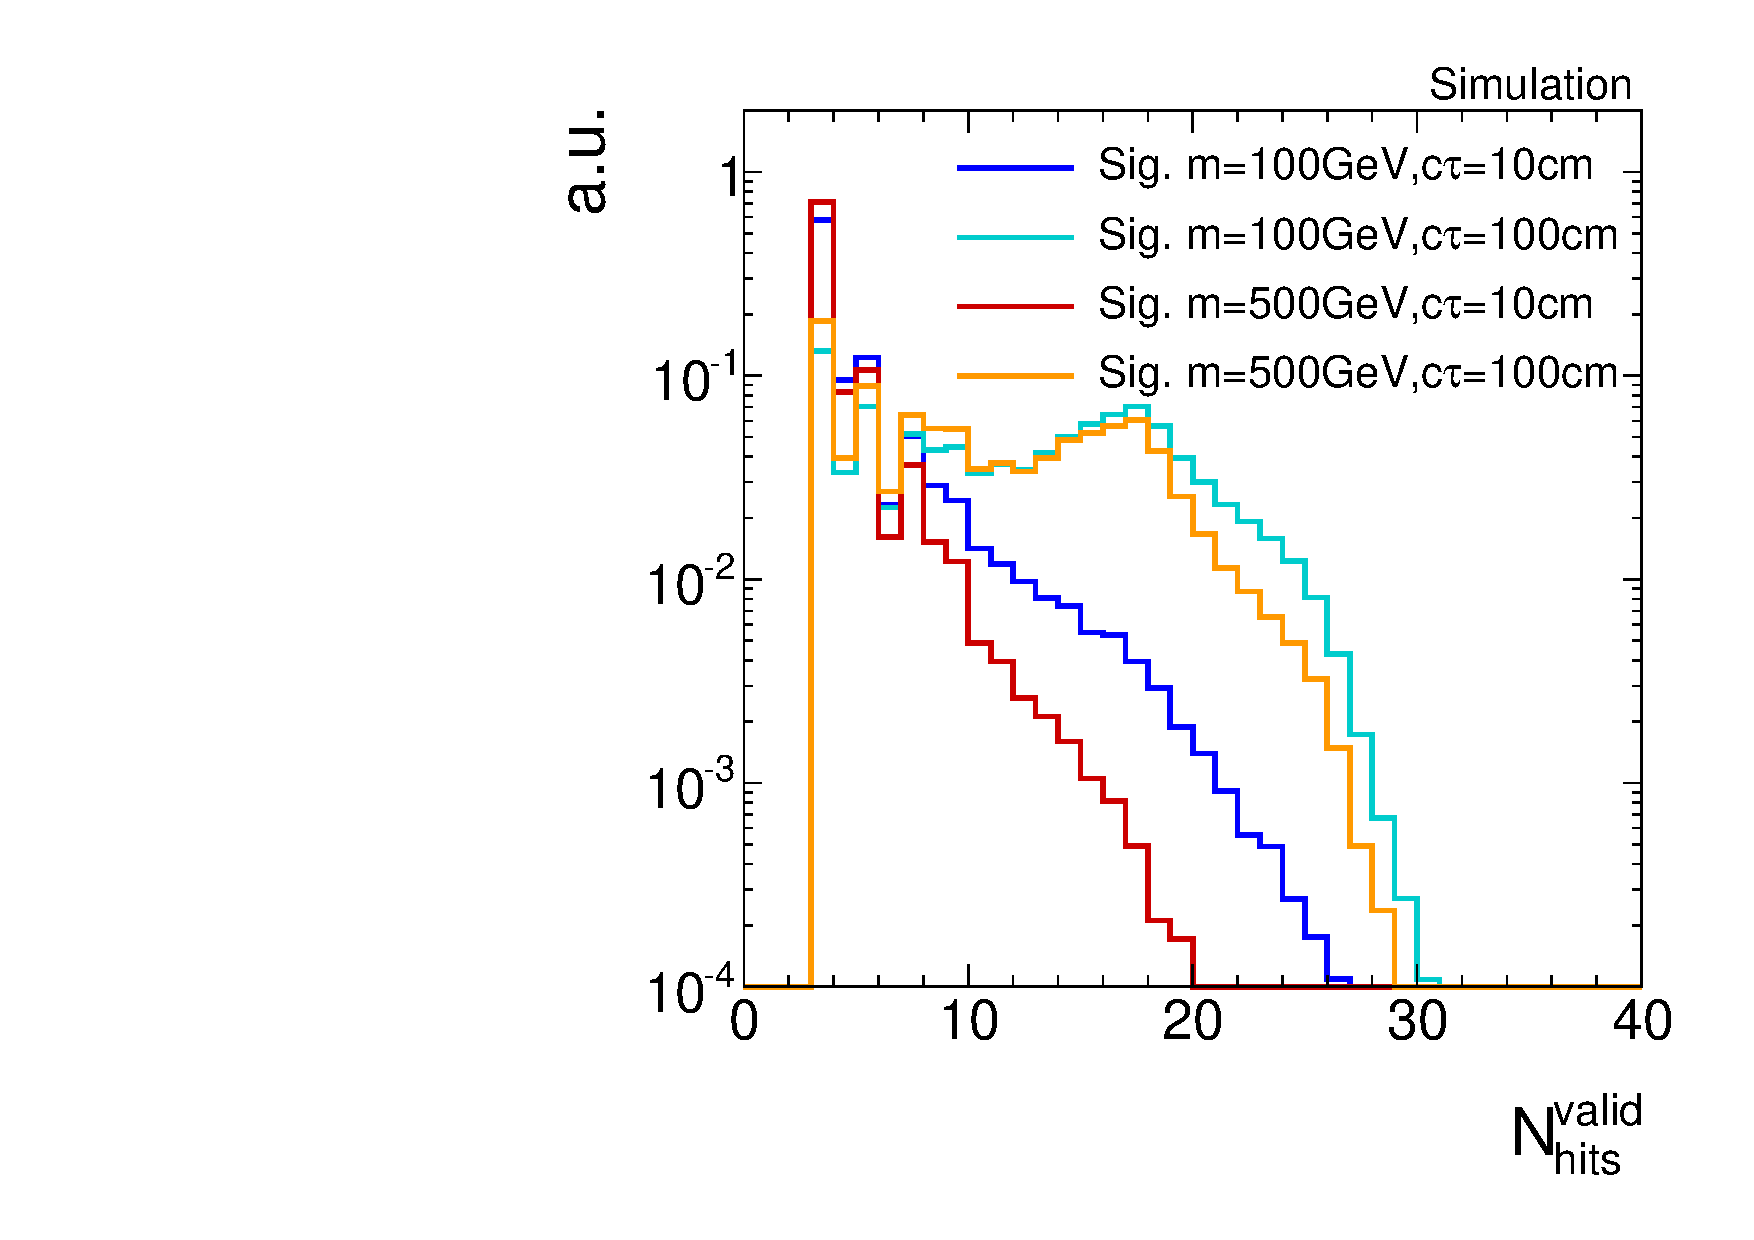
\includegraphics[width=0.49\textwidth]{figures/analysis/MotivationAndGeneralSearchStrategy/htrackNValid_log_chiTracksnoSelection.pdf}
  %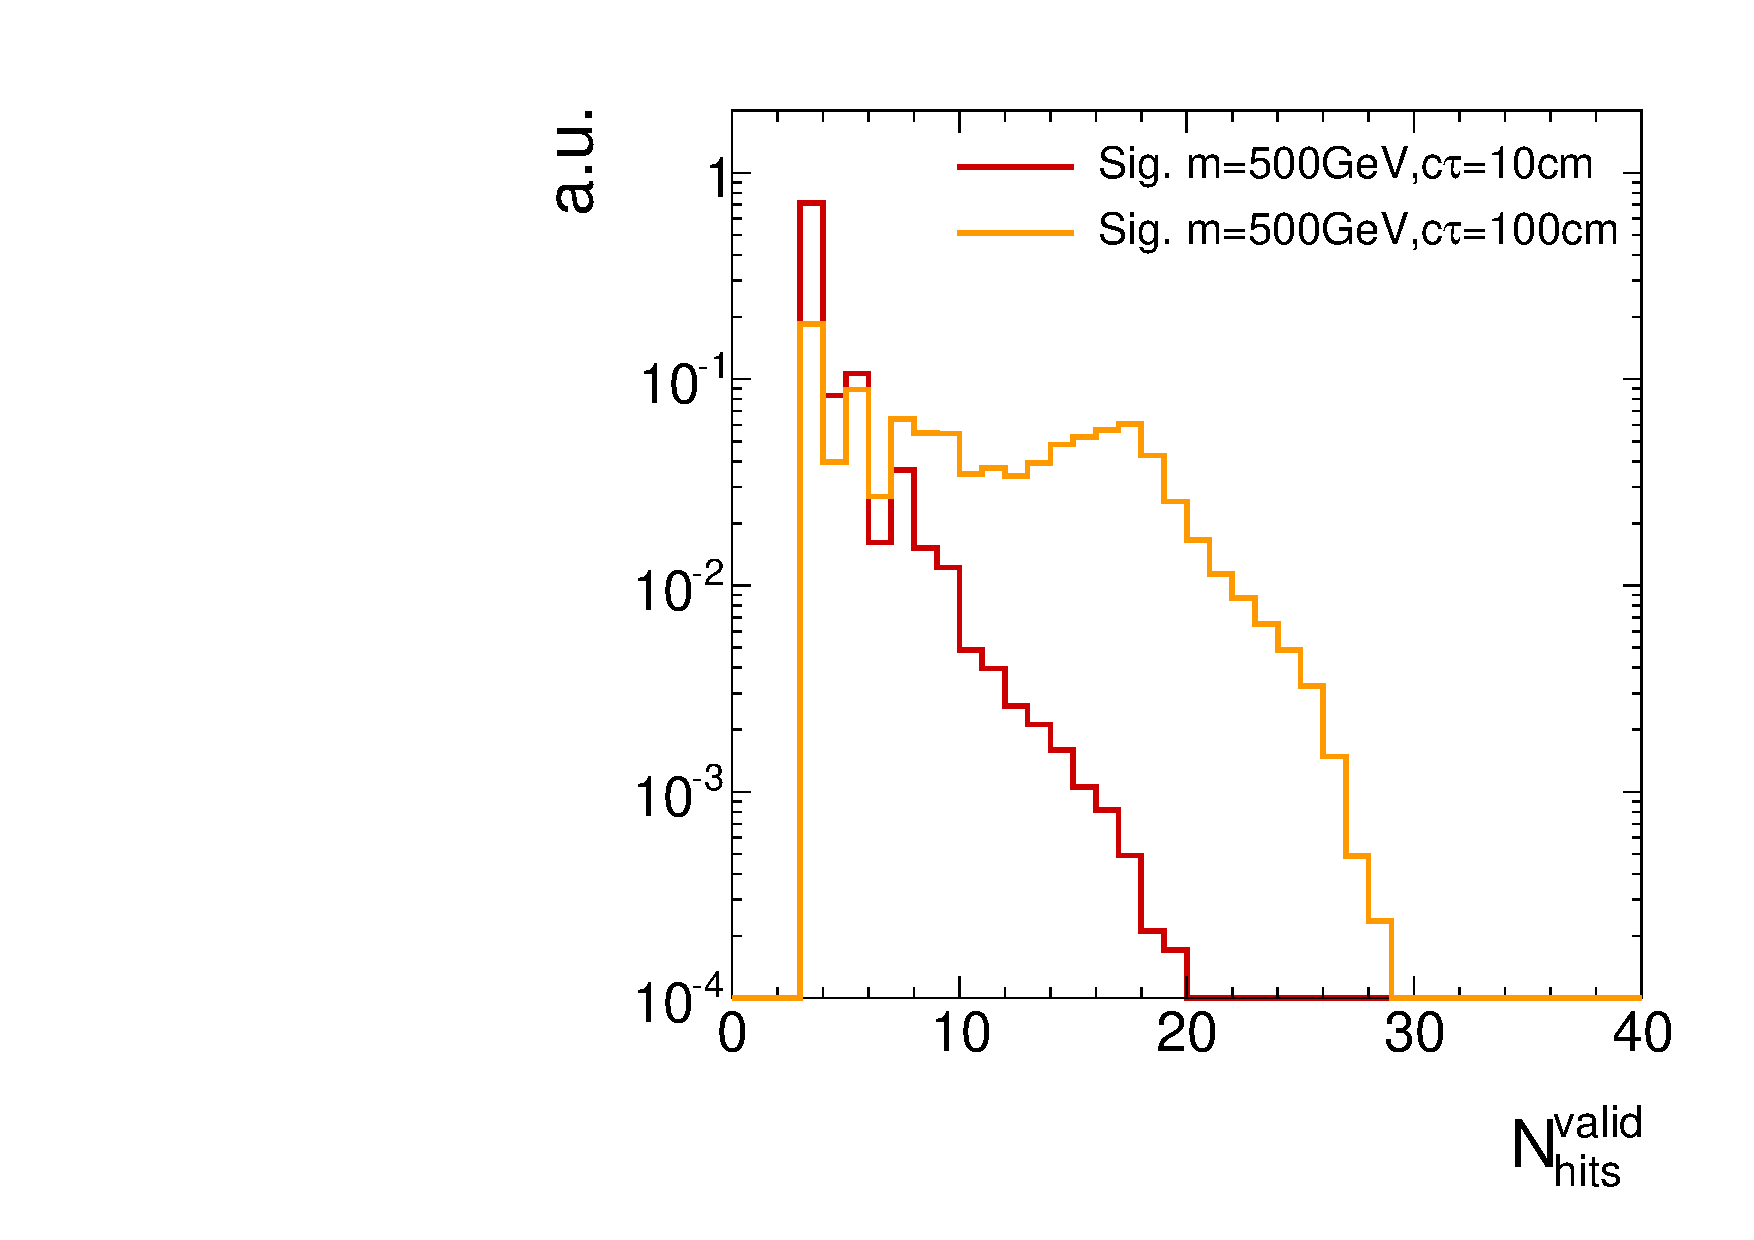
\includegraphics[width=0.49\textwidth]{figures/analysis/htrackNValid_log_chiTracksnoSelection_m500GeV.pdf}
  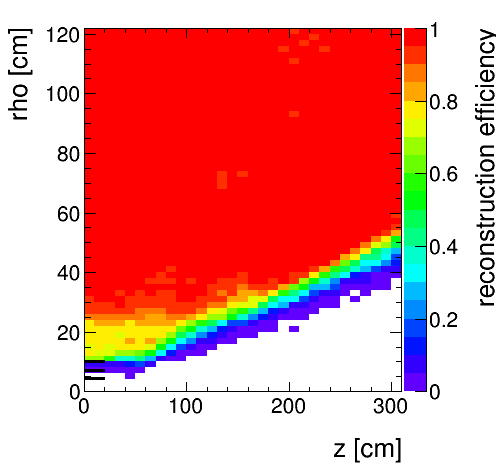
\includegraphics[width=0.49\textwidth]{figures/analysis/MotivationAndGeneralSearchStrategy/RecoEffTracksZoom.png}
  \end{tabular}
  \caption{Left: Number of measurements in the tracker system \nhits for four different signal lifetimes.
                 The low lifetime samples are rapidly falling and peaking at the lowest number of possible measurements of three. 
                 For a lifetime of $\ctau=50\cm$, a second peak at $\sim$17 hits appears corresponding to the number of measurements when crossing all pixel barrel (3) and strip inner and outer barrel (6 from stereo and 8 from normal) layers.
           Right: Probability to reconstruct a track (z) in dependency of the chargino's decay point (x and y).
           More information on the generation of the simulated signal samples can be found in Section~\ref{sec:SignalSamples}}. 
  \label{fig:NHits_2Signal_noSelection_normalized}
\end{figure}



Additionally, the search for disappearing tracks which targets models with charginos decaying inside the tracker did not make use of the high energy deposition of heavy particles. 
Although this variable was indeed used in the search for long-lived charged particles, this search was not optimised for intermediate lifetimes (e.g. no explicit muon veto on the selected tracks was required). 
Thus, it shows less sensitivity compared to the disappearing track search in the lifetime region between $35\,\text{cm} \lesssim c\tau \lesssim 100\,\text{cm}$ (see Fig.~\ref{fig:pMSSMplot}).\\

To conclude, the general search strategy of the here presented analysis is to unite the strategies of \cite{bib:CMS:HSCP_8TeV} and \cite{bib:CMS:DT_8TeV} and to lower the strong selection on the number of hits in these analyses in order to get an optimised selection for lifetimes around $10\,\text{cm} \lesssim c\tau \lesssim  40\,\text{cm}$.

%%%%%%%%%%%%%%%%%%%%%%%%%%%%%%%%%%%%%%%%%%%%%%%%%%%%%%%%%%%%%%%%%%%%%%%%%%%%%%%%%%%%%%%%%%%%%%%%%%%%%%%%%%%%%%%%%%%%%%%%%%%%%%%%%%%%%%%%%%%%%%%%%%%%%%%%%%%%%%%%%%%%%%%%%%%%%%%%%%%%
%%%%%%%%%%%%%%%%%%%%%%%%%%%%%%%%%%%%%%%%%%%%%%%%%%%%%%%%%%%%%%%%%%%%%%%%%%%%%%%%%%%%%%%%%%%%%%%%%%%%%%%%%%%%%%%%%%%%%%%%%%%%%%%%%%%%%%%%%%%%%%%%%%%%%%%%%%%%%%%%%%%%%%%%%%%%%%%%%%%%
\chapter{Improved dE/dx measurement of short tracks}
\label{sec:DeDxMeasurement}
The CMS tracker system does not only allow for the precise measurement of particle's tracks and primary and secondary vertices but also the measurement of a particle's energy loss within the tracker material.
This is done by the detection of the number of electrons produced by the ionisation of the particle during its passage through the silicon tracker.
A detailed introduction to the CMS tracker system and the energy measurement can be found in Section~\ref{FIXME}.

It was already pointed out that the inclusion of the pixel energy measurements can increase the sensitivity when searching for short tracks.
While the silicon strip detector has already been calibrated as part of the search for long-lived charged particles \cite{bib:CMS:HSCP_8TeV}, no offline calibration has been done for the pixel silicon tracker so far.
To increase the discrimination power of $dE/dx$ for short tracks, such a calibration procedure was therefore conducted within this PHD thesis.


\section{Ionisation loss of charged particles}
\label{sec:sub:MeasuringDeDx}
The mean energy loss per path length of particles travelling through a layer of material can be described with the Bethe formula \cite{bib:Bethe_1930}:
\begin{equation*}
\langle \frac{dE}{dx} \rangle = Kz^2\frac{Z}{A}\frac{1}{\beta^2} [ \frac{1}{2} \ln{\frac{2m_e c^2 \beta^2 \gamma^2 T_{\text{max}}}{I^2}} - \beta^2 - \frac{\delta( \beta \gamma )}{2} ].
\end{equation*}
It is valid if the main energy loss originates from ionisation effects, i.e. in a region between $0.1\lesssim\beta\gamma\lesssim 1000$.
It is a function of the atomic number ($Z$) and the atomic mass ($A$) of the absorber. 
The mean excitation energy ($I$) for silicon is 173\,eV \cite{bib:NIST}. 
$T_{\text{max}}$ represents the maximum energy transfer in a single collision.
The relevant particle's properties are the velocity ($\beta$), the Lorentz factor ($\gamma$) and the charge (z) of the incident particle.
The density correction $\delta( \beta \gamma )$ reduces the mean energy loss at high energies because of polarisation effects of the material. 
The constant factor K is $4\pi N_A r_e^2 m_e^2 c^2$ with $N_A$ being the Avogadro’s number.

Even if widely used, the mean energy loss is a quantity which is ``ill-defined experimentally and is not useful for describing energy loss by single particles'' \cite{bib:PDG_2014}.
The problem is caused by the underlying probability distribution of one single $dE/dx$ measurement (this will be named $\Delta E/ \Delta x $ throughout the following sections), which can be parametrised by a Landau distribution \cite{bib:Landau_1944}
\begin{equation*}
p(x) = \frac{1}{\pi} \int_0^\infty\! e^{-t \log t - x t} \sin(\pi t)\, dt.
\end{equation*}
The Landau distribution has no free parameters. Its most probable value is around 0.222.
However, it is possible to introduce artifically a different most probable value and a width with $x \rightarrow \frac{x-\text{MPV}}{\sigma}-0.222$.
The Landau distribution is a highly asymmetric distribution with a long tail towards the right end (see Fig.~\ref{fig:landau}).
Theoretically it extends to infinite energies, however in nature the maximal deposited energy is of course limited by the particle's full energy.
The mean and the variance of a landau distribution are not defined.
Because of its strong asymmetry, measurements of $\langle dE/dx \rangle$ with only a few single measurements are easily biased towards high values, making the mean energy loss described by the Bethe formula a problematic and unstable concept. 
%This is again different for a (limited) measurment, as there it is always possible to calucalute a mean.
%Still, this leads to the fact that the definition of the mean energy loss per path length is a problematic and unstable concept.


A much better observable is the most probable value (MPV): the maximum of the Landau distribution.
The MPV is much more stable compared to the mean and is not as easily biased towards higher $dE/dx$ values. 
The most probable energy loss of a charged particle, $\Delta_p$, is defined by the Landau-Vavilov-Bichsel equation \cite{bib:Bichsel:MPV_1988}:
\begin{equation}
\Delta_p = \xi \left[ \ln \frac{2mc^2\beta^2\gamma^2}{I}  + \ln\frac{\xi}{I} + j - \beta^2 - \delta(\beta\gamma)  \right],
\label{eq:Landau_Vavilov_Bichsel}
\end{equation}
with $\xi=(K/Z)\langle Z/A \rangle (x/\beta^2)$. 
The thickness of the absorber $x$ appears explicitly in the Landau-Vavilov-Bichsel equation making the most probable energy loss per path \mbox{length $\Delta_p/dx$} logarithmically dependent on $x$.
A comparison between the Bethe mean energy loss $\langle dE/dx \rangle$ and the most probable energy loss $\Delta_p/dx$ is shown in Fig.~\ref{fig:dEdx_Bethe_Landau}.
\begin{figure}[!b]
  \centering 
  \begin{tabular}{c}
  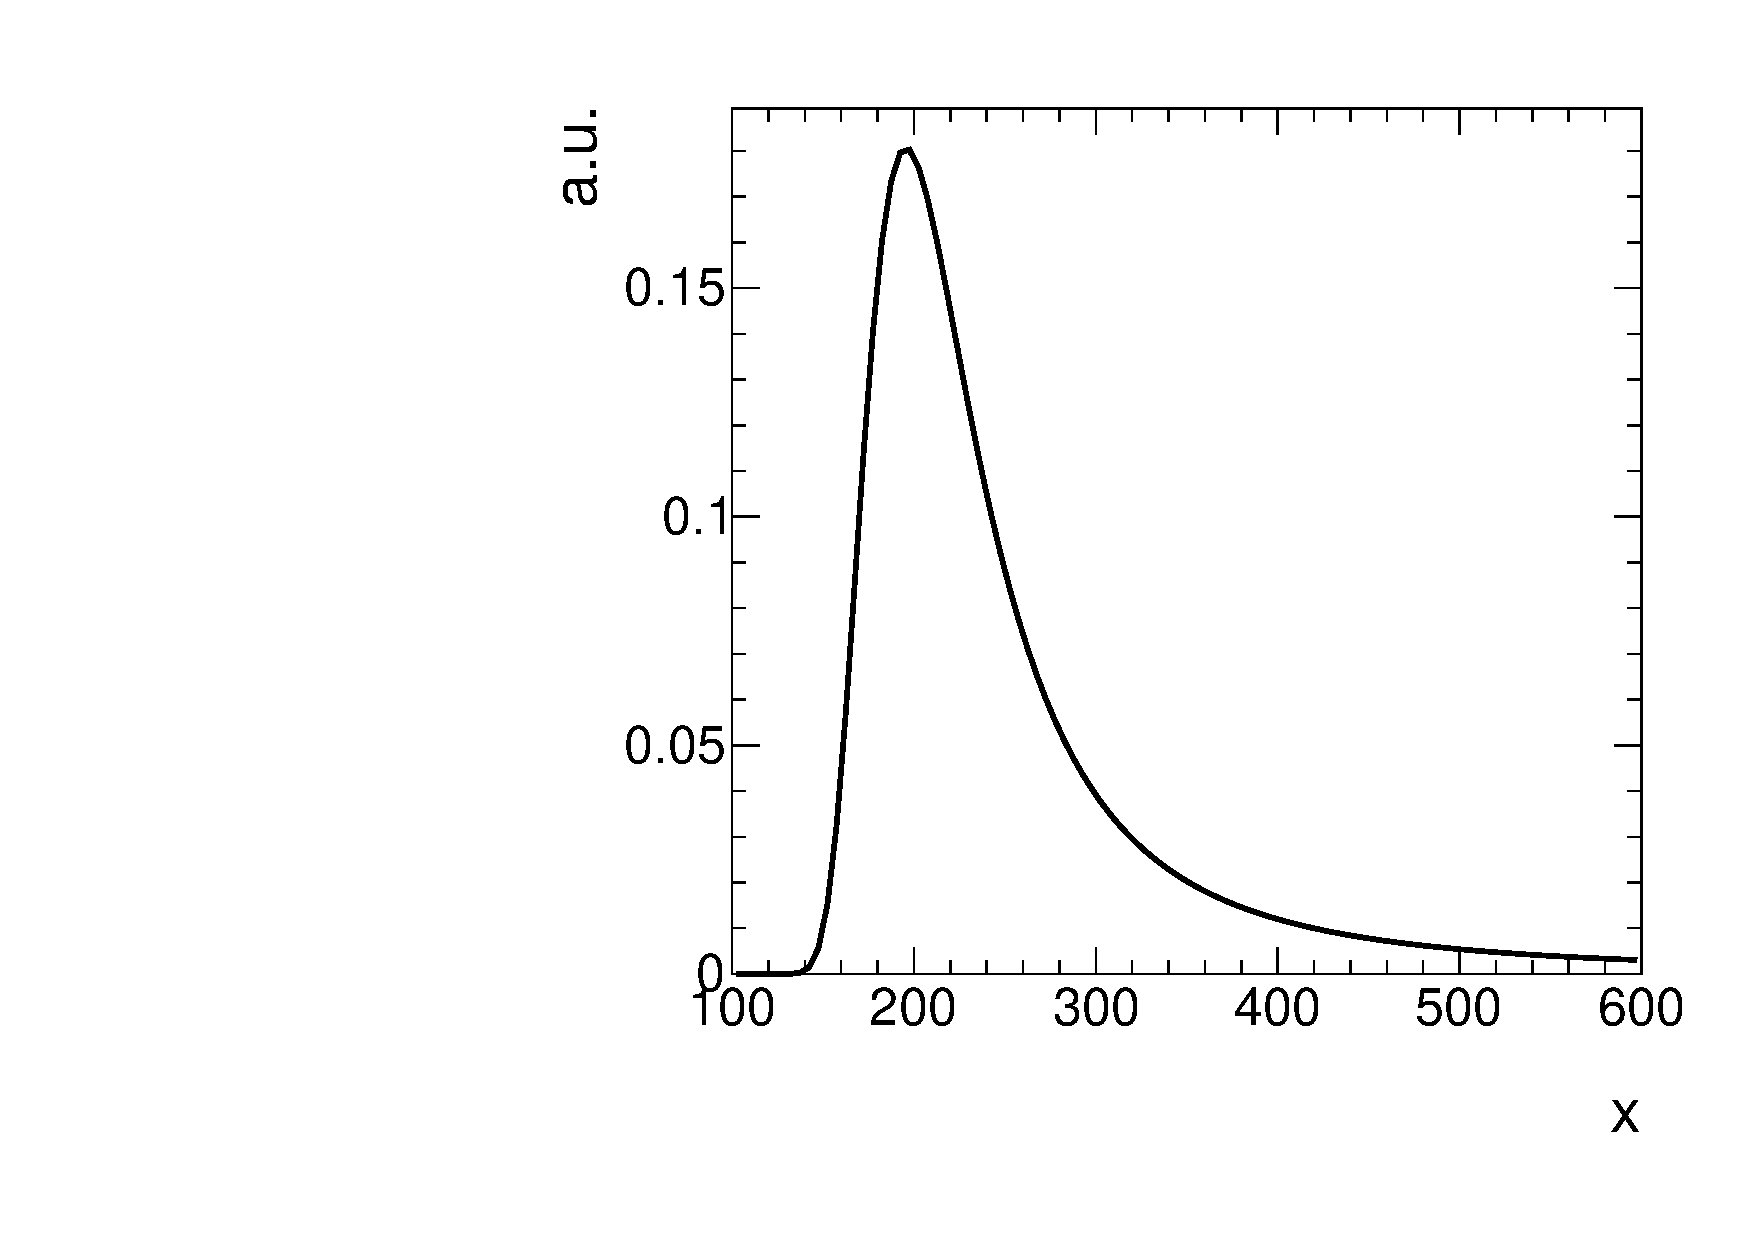
\includegraphics[width=0.49\textwidth]{figures/analysis/PixelCalibration/Landau.pdf}
  \end{tabular}
  \caption{Illustration of the shape of a Landau distribution. Parameters were chosen as $\mu=200$ and $\sigma=20$.} 
  \label{fig:landau}
\vspace{92pt}
\end{figure}
\begin{figure}[!bt]
  \centering 
  \begin{tabular}{c}
  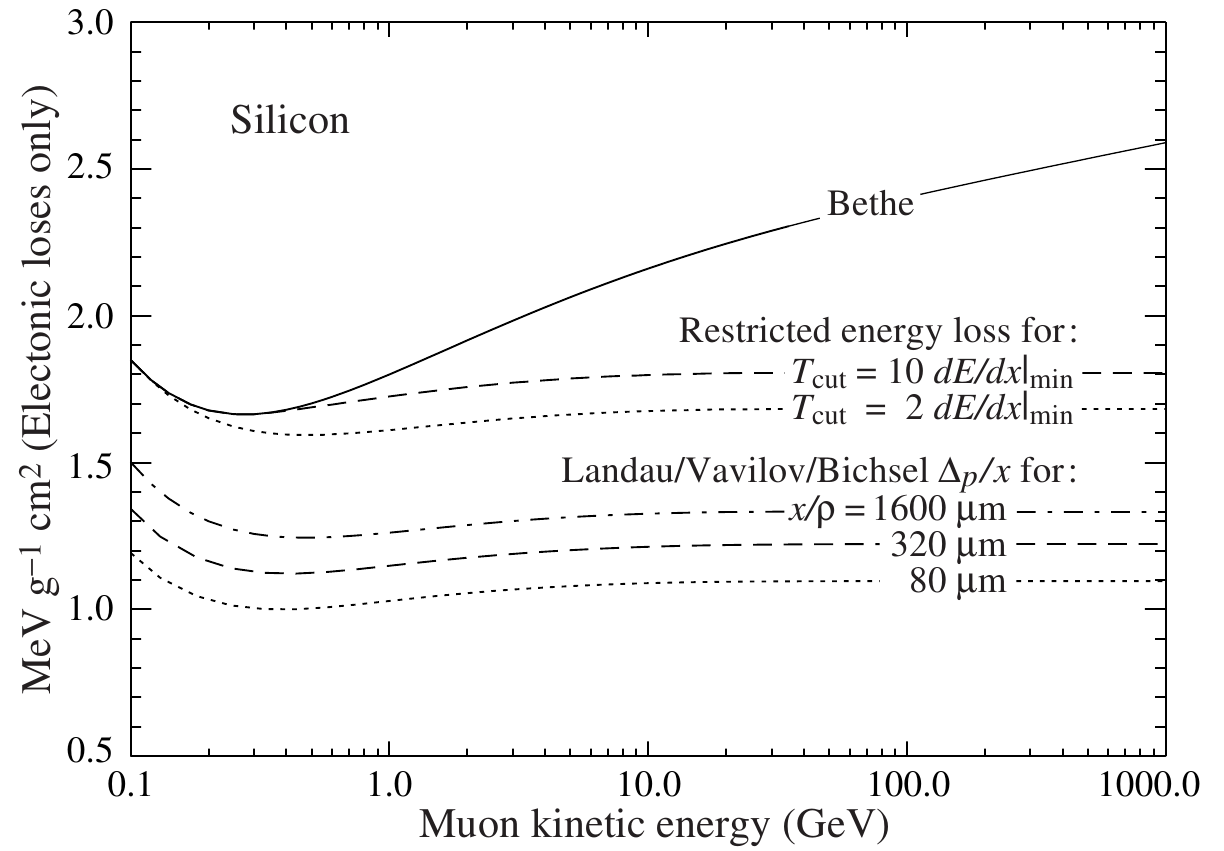
\includegraphics[width=0.6\textwidth]{figures/analysis/dEdx_Bethe_Landau.png}
  \end{tabular}
  \caption{Comparison between the Bethe mean energy loss, restricted energy loss and the most probable energy loss described by the Landau-Vavilov-Bichsel function for muons for different values of absorber thickness. 
           Taken from \cite{bib:PDG_2014}.} 
  \label{fig:dEdx_Bethe_Landau}
\end{figure}
However, it is difficult to determine the most probable value for tracks with only $\sim$15 energy measurements available.
Large fluctuations can still lead to a bias towards higher value of the most probable $dE/dx$.

Several "estimators'' exist that suppress a potential bias towards the high end without introducing a bias towards lower values~\cite{bib:Quertenmont_2010}.
One of the estimators, also used in the next chapter, is the harmonic-2 estimator
\begin{equation}
\ihtwo=\left( \frac{1}{N}\sum_{i=1}^{N}(\Delta E/\Delta x)_i^2 \right)^{-1/2},
\label{eq:Harmonic2Estimator}
\end{equation}
where $\Delta E /\Delta x$ corresponds to one measurement in one tracker module. 
The harmonic mean of all $N$ measurements to the power of two is the estimated most probable $dE/dx$.\\

SM particles such as pions and muons are minimally ionising in silicon for $\beta\gamma \sim 3-4$ (see Fig.~\ref{fig:dEdx_Landau_Silicon}). 
For higher momenta the deposited energies increase again reaching a plateau at around $\beta\gamma\sim100$. 
However, new heavy charged particles would mainly be unrelativistic because of their high mass and would therefore deposit much higher energies in the detector.
This makes $dE/dx$  a very well discriminating variable.
\begin{figure}[!bt]
  \centering 
  \begin{tabular}{c}
  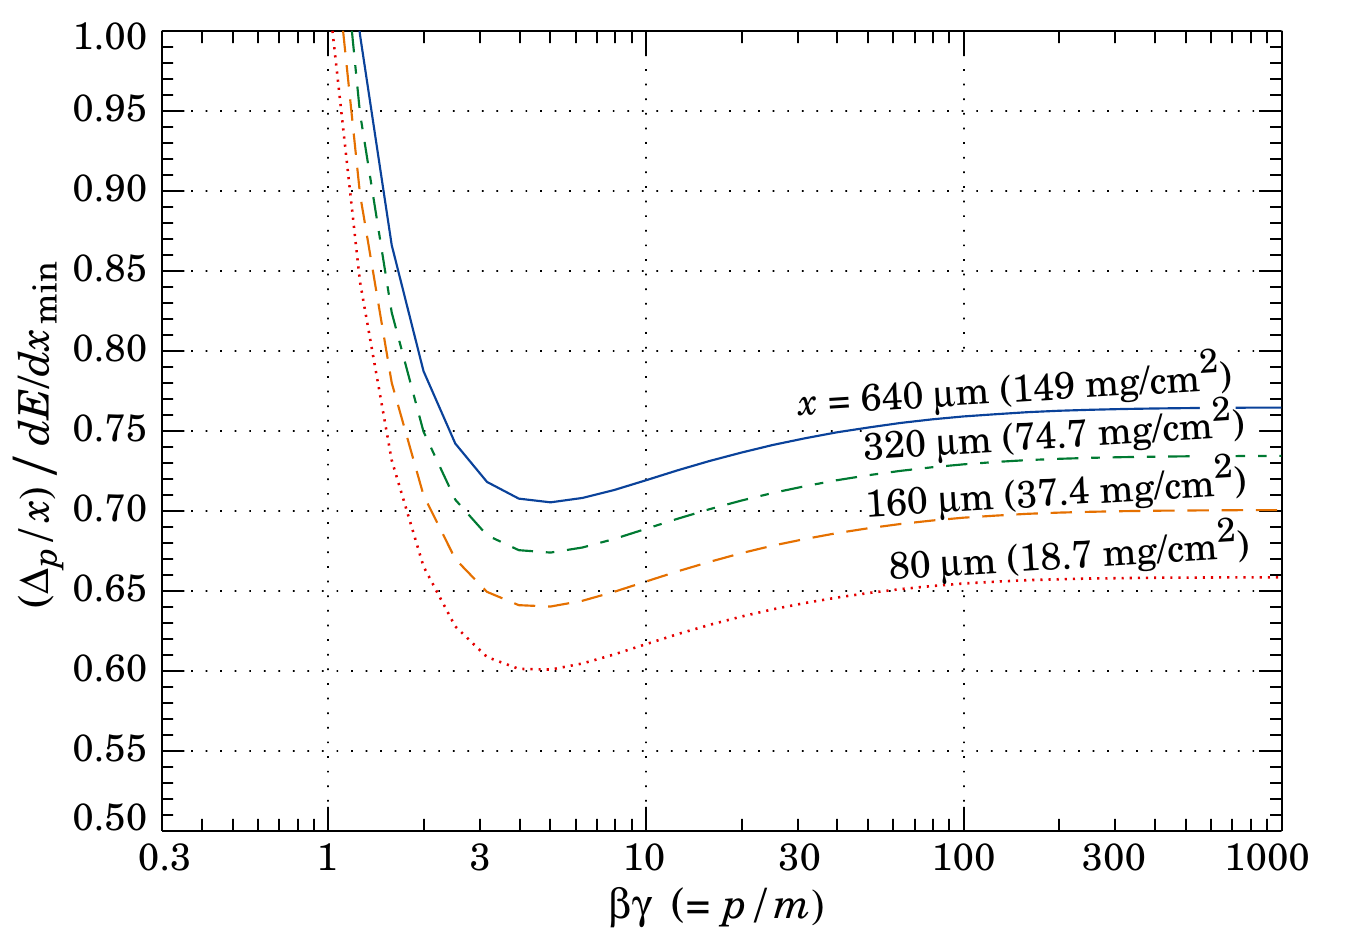
\includegraphics[width=0.6\textwidth]{figures/analysis/dEdx_Landau_Silicon.png}
  \end{tabular}
  \caption{Most probable energy loss in silicon, scaled to the mean loss of a minimally ionising particle (388 eV/$\mu$m) for different absorber thicknesses. Taken from \cite{bib:PDG_2014}.} 
  \label{fig:dEdx_Landau_Silicon}
\end{figure}
Thus, the energy loss per path length can be used to discriminate between SM particles and new heavy charged particles, which are usually unrelativistic because of their high mass.

\section{Energy calibration of the silicon pixel tracker}
During Run I in 2012, the pixel silicon detector was continuously subjected to an energy calibration, a so-called gain calibration~\cite{bib:Danek}.
Every pixel was calibrated to the same response, so that the whole pixel tracker should have been well inter-calibrated.
Unfortunately, due to various reasons, such as the imperfect constancy of the reference signal, or radiation and temperature induced changes, the energy calibration could not ensure a fully calibrated pixel tracker.
%was not adequate enough to use the measured energy deposition without a further offline calibration procedure.
This imperfection of the gain calibration can be seen in Fig.~\ref{fig:StabilityPlot_beforeCalibration}, where the sum of the harmonic-2 estimator for all tracks $\sum\limits_{\text{all trks}}\ihtwo$ over the full data-taking period in 2012 is shown.
Four different steps can be spotted.
\begin{figure}[!t]
  \centering 
  \begin{tabular}{c}
  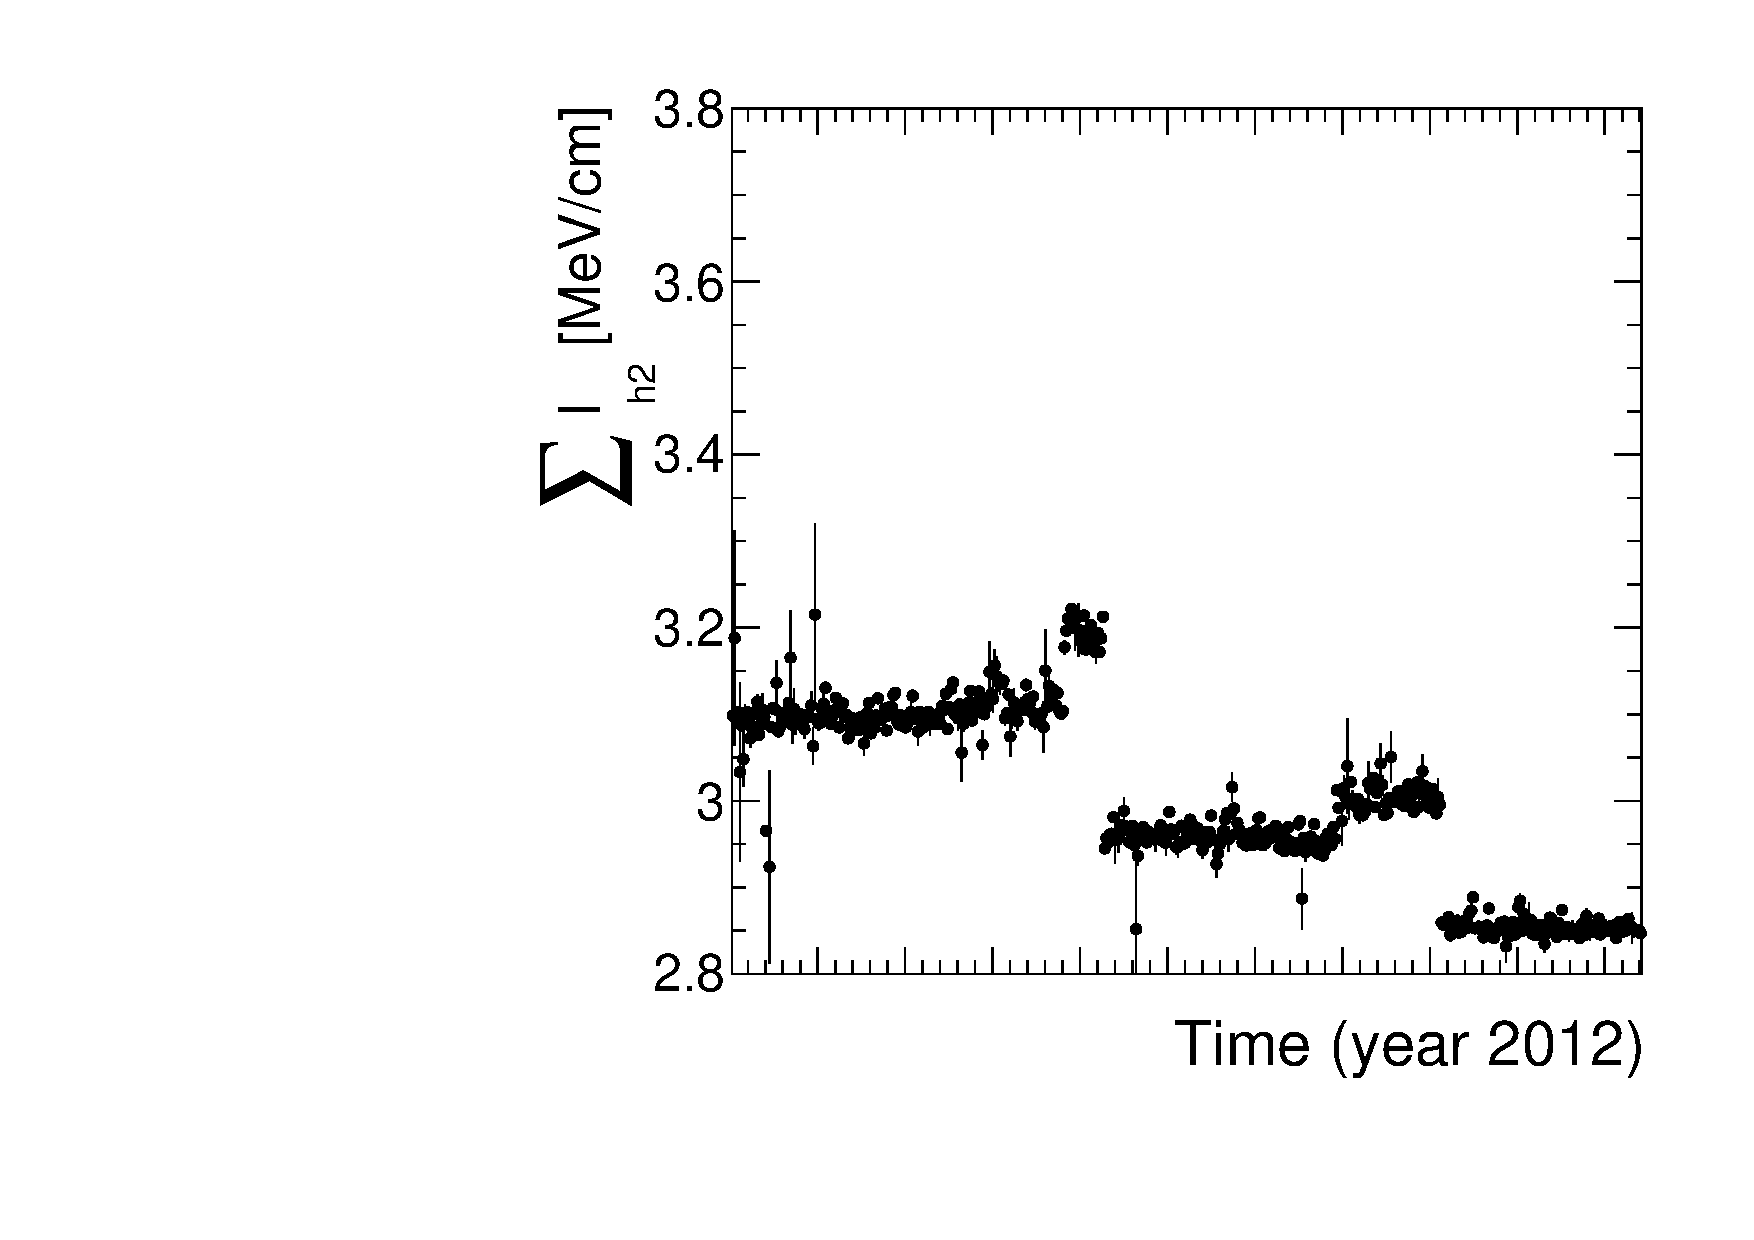
\includegraphics[width=0.49\textwidth]{figures/analysis/PixelCalibration/StabilityPlot_Pixel_beforeCalibration_withoutStepFits_NEW.pdf}
  \end{tabular}
  \caption{Sum of all track's $dE/dx$ (harmonic-2 estimator) over the full year 2012. Only pixel hits are taken into account. Every data point corresponds to one run.} 
  \label{fig:StabilityPlot_beforeCalibration}
\end{figure}
The first and the third steps correspond to changes in the settings of the tracker due to irradiation.
The second and fourth step are induced by associated adjustments in the online gain calibration.
Unfortunately, although the gain calibration was adjusted (even with some delay), it was not able to ensure a constant energy response of the pixel tracker over time. 
The variations of the dE/dx measurement over time of around 15\% is too large to use dE/dx without a further calibration. 

The following sections explain the method of the gain calibration of the pixel silicon tracker which was conducted for this analysis. 
It is splitted into a section about the inter-calibration of gain and the absolute calibration of gain) 
Detailed technical information about the pixel tracker can be found in Section~\ref{sec:Detector:Pixel}.


\subsection*{Inter-calibration of gain}
The main goal of the gain calibration is to get a uniform response in the ionisation energy loss $dE/dx$ over the full data taking period in 2012.
To also ensure a uniform response of all modules within one time step, an additional inter-calibration on module level was carried out.
The inter-calibration can in principle be done on various levels: the highest granularity would be a calibration on pixel level, followed by a calibration on read-out-chip (ROC) level and then on module-level.
Lower granularities in descending order are rings (modules with same z-position) and finally layers (3 layers in the barrel and 4 disks in the endcap). 
It was checked that all pixels and all ROCs (on one module) are well inter-calibrated, such that the inter-calibration was finally done module-wise.
%The applied method for the gain calibration of the pixel tracker closely follows the method in \cite{bib:Quertenmont_2010}.

The gain calibration of the pixel silicon tracker has been carried out with the help of minimally ionising particles (MIPs).
MIPs in this context are not defined as particles depositing a minimum amount of energy, but more generally a small amount of energy.
This denotes all particles located at the plateau of the $dE/dx$ distribution vs. momentum (see Fig.~\ref{fig:dEdx_Landau_Silicon}).
This approach ensures that all particles deposit similar amount of energy so that the variation due to different momenta is minimised.
MIPs are selected by a momentum selection of $\text{p}>2\,$\gev.
Additionally, only tracks with at least eight hits and a $\chi^2/\text{n.d.o.f.}<3$ are used to ensure a high-quality track reconstruction.
A sample containg around $~$50 million ``minimum bias'' events is used for calibration.
The ``minimum bias'' sample was specifically recorded for tracker calibration purposes.
Its distinctive property is that neither an online nor offline selection was applied.

For every module in the pixel tracker (there are 1440 modules in total), a distribution of the energy loss per path length $\Delta E/\Delta x$ is built.
The measurement of $\Delta E/\Delta x$ is done in ADC counts per mm.
ADC counts are a measure for the deposited charge after digitisation.
%each $\Delta E/\Delta x$  measurement of all particles crossing the module is filled into a histogram. 
Figure~\ref{fig:dEdx_Module} shows an example distribution for one module.
\begin{figure}[!bt]
  \centering 
  \begin{tabular}{c}
  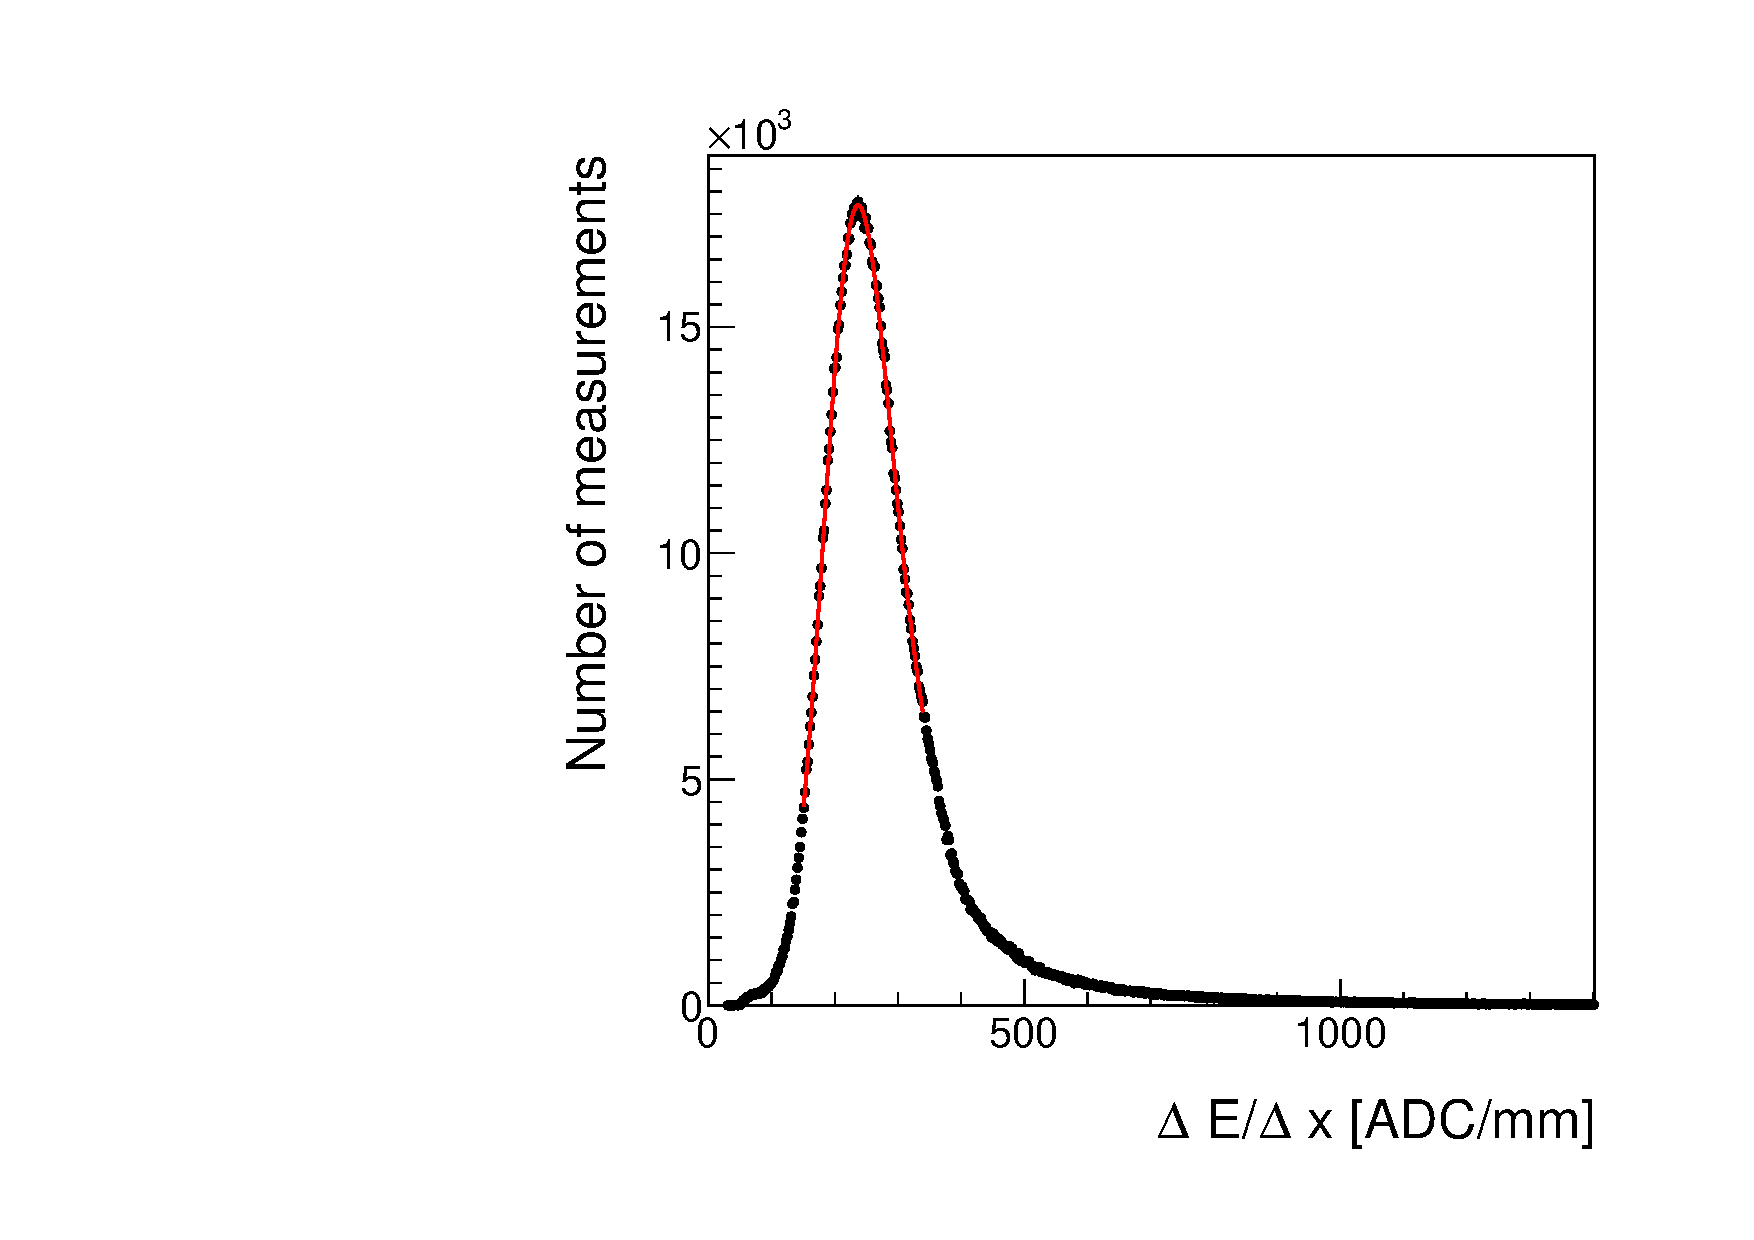
\includegraphics[width=0.49\textwidth]{figures/analysis/Landau_Module_352476680.pdf}
  \end{tabular}
  \caption{An example of the $\Delta E/\Delta x$ distribution measured in ADC count per mm for one module of the CMS pixel tracker. 
           A Landau convoluted with a Gaussian is fitted to the core of the distribution in an iterative procedure.} 
  \label{fig:dEdx_Module}
\end{figure}
The underlying Landau distribution can be nicely seen. 
To extract the MPV for every module a fit to the core distribution is performed.
The fit is done with a Landau convoluted with a Gaussian function to be closer to the experimentally observed energy spectrum.
This also increases the fit performance and the stability of the fit.
The path length $\Delta x$ is calculated with
\begin{equation*}
\Delta x = d_{\text{module}_i} \cdot \cos(\phi_{\text{track}}),
\end{equation*}
where $d_{\text{module}_i}$ is the thickness of module i and $\phi_{\text{track}}$ is the relative angle of the particle's trajectory to the normal axis of the module.
With the measured MPV extracted from the fit, an inter-calibration factor is calculated for every module
\begin{equation*}
c_{\text{inter}}=\frac{\mpv_{\text{target}}\, [\text{ADC/mm}]}{\mpv\, [\text{ADC/mm}]} = \frac{300 \cdot 265 \, \text{ADC/mm}}{\mpv\, [\text{ADC/mm}]}.
\end{equation*}
The factor 300 $\cdot$ 265 ADC/mm is in principal an arbitrary number since the final response is adjusted by the absolute gain calibration described in the next section.
However, it was chosen such that it corresponds approximately to the most probable energy deposition of a MIP.
The calibration factor can then be used to scale every single measurement in a module to a calibrated $\Delta E/\Delta x$ measurement
\begin{equation*}
\frac{\Delta E}{\Delta x}_{\text{calibrated}}=c_{\text{inter}} \cdot \frac{\Delta E}{\Delta x}_{\text{uncalibrated}}
\end{equation*}
The determination of the calibration factor needs to be done for every of the five time steps, shown in Fig.~\ref{fig:StabilityPlot_beforeCalibration} independently, in order to get rid of the time dependency. 
The result of the inter-calibration can be seen in Fig.~\ref{fig:StabilityPlot_afterCalibration}.
The variation over time was indeed eradicated, resulting in a maximal time variation of less than $\sim1$\%.
\begin{figure}[!bt]
  \centering 
  \begin{tabular}{c}
  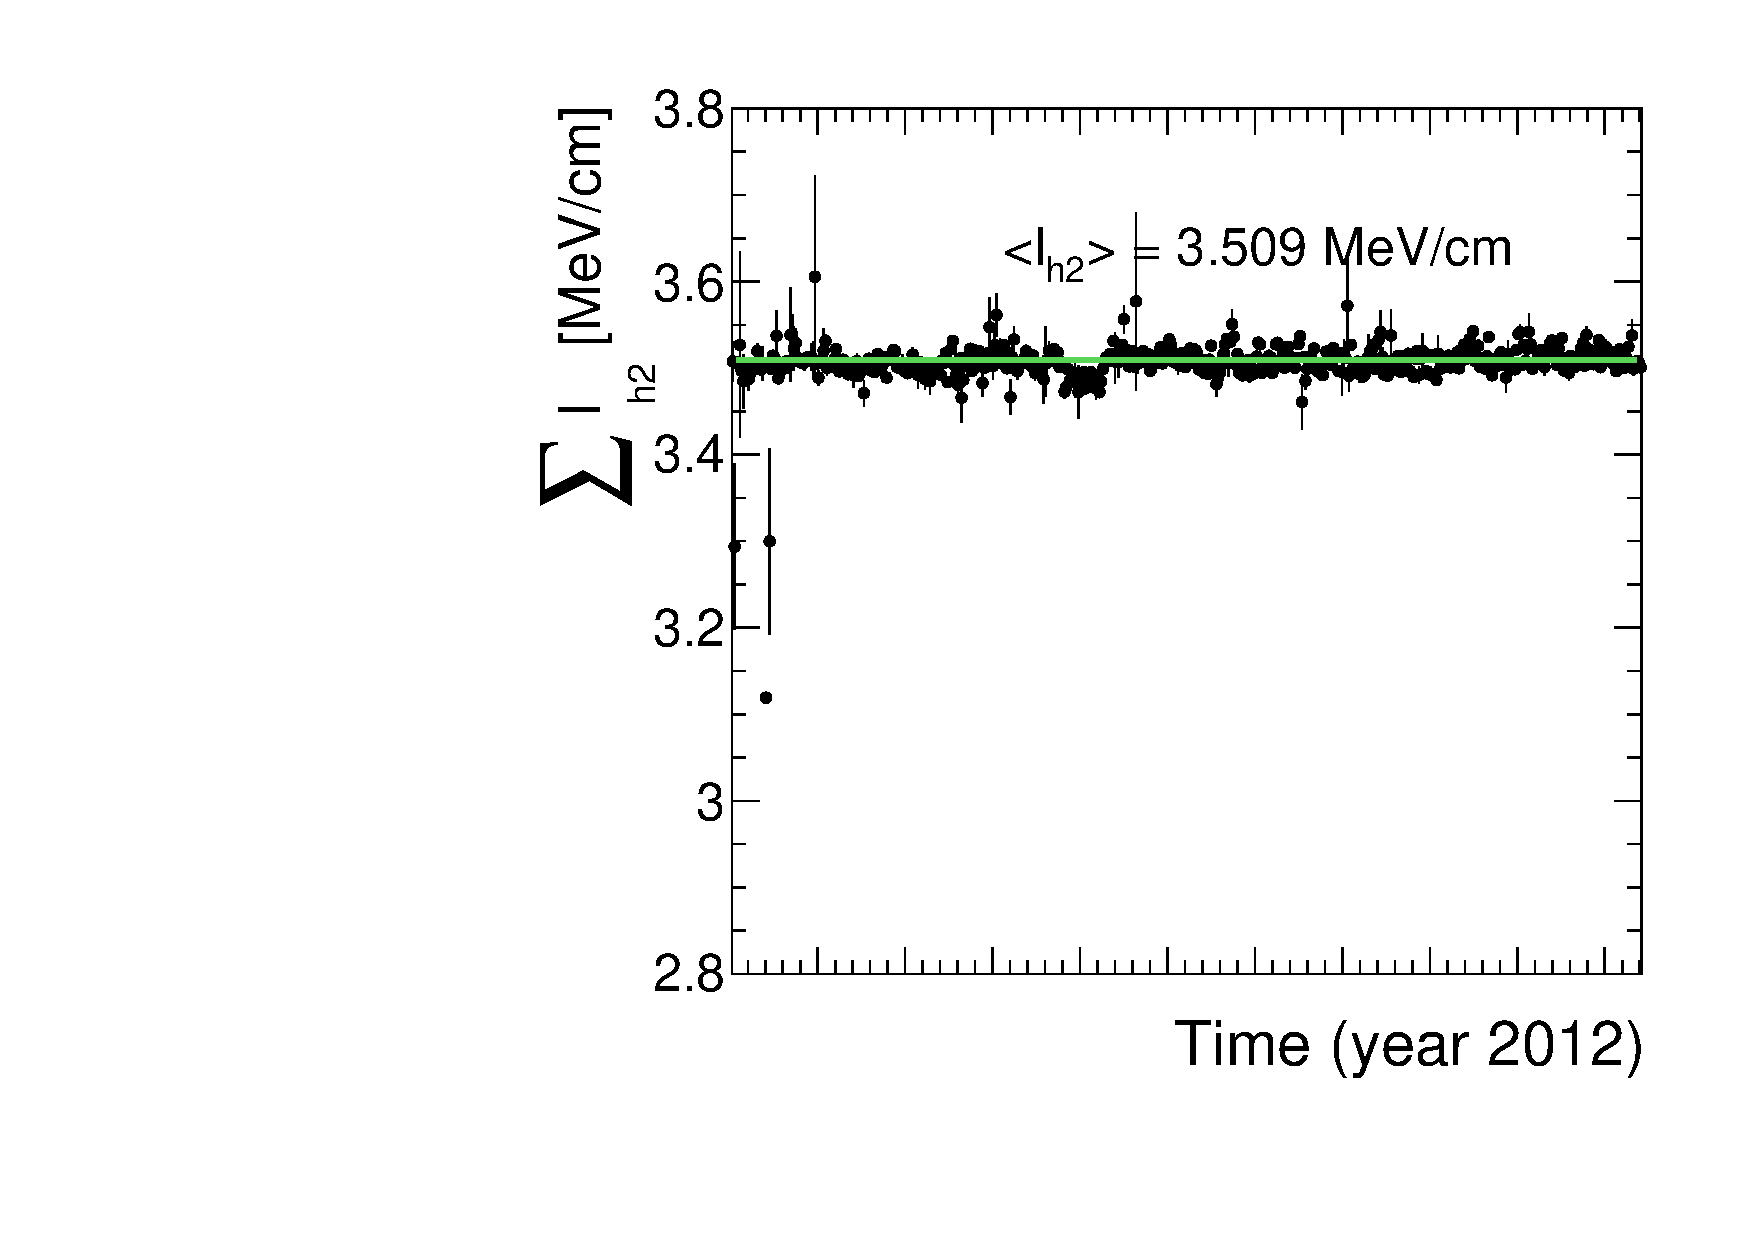
\includegraphics[width=0.49\textwidth]{figures/analysis/PixelCalibration/StabilityPlot_Pixel_afterCalibration_withoutStepFits_NEW.pdf}
  \end{tabular}
  \caption{Sum of all track's $dE/dx$ (harmonic-2 estimator) over the full year 2012 after applying the calibration factors, resulting in an average $dE/dx$ of 3.51 MeV/cm. Only pixel hits are taken into account. Every data point corresponds to one run.} 
  \label{fig:StabilityPlot_afterCalibration}
\end{figure}

Additionally, the same procedure is carried out for a corresponding simulated data sample to ensure the inter-calibration of the pixel modules on all simulated samples.




\subsection*{Absolute calibration of gain}
As a final step, the targeted \mpv being $\mpv_{\text{target}}=300 \cdot 265 \,  \text{ADC/mm}$ needs to be translated to a meaningful physical quantity given in physical units (e.g. MeV/cm).
That means, that the charge measurement in ADC counts needs to be converted to the real energy release of a particle.
The relation between $\Delta E$ in ADC counts and the energy loss in eV is given by
\begin{equation*}
\Delta E\,[\ev] = c_{\text{inter}} \cdot \Delta E\,[\text{ADC}] \cdot \frac{N_e}{\text{ADC}} \cdot 3.61 \, \ev,
\end{equation*}
where $N_e$/ADC is the number of electrons which correspond to one ADC count and 3.61\,\ev is the  mean energy needed to create one electron-hole pair in silicon at -10$\degree$C.
Such an absolute gain calibration can be done with the help of several methods (all explained in \cite{bib:Quertenmont_2010}).
The absolute calibration of the silicon pixel tracker can rely on the already conducted absolute calibration of the silicon strip detector.
In \cite{bib:Quertenmont_2010}, the absolute gain calibration was done with the help of the most probable energy release per path length of muons, 
theoretically described by the Landau-Vavilov-Bichsel formula in Eq.~\ref{eq:Landau_Vavilov_Bichsel}.  
To calibrate the pixel tracker to the correct energy loss per path length it is therefore sufficient to determine one calibration factor to relate the average $dE/dx$ of all tracks in the pixel tracker as shown in 
Fig.~\ref{fig:StabilityPlot_afterCalibration} to the average measured $dE/dx$ in the strip tracker, shown in Fig.~\ref{fig:StabilityPlot_Strip} by
\begin{equation*}
c_{\text{absolute}} = \frac{dE/dx_{\text{strip}}}{dE/dx_{\text{pixel}}} = \frac{3.303}{3.509} = 0.941.
\end{equation*}
\begin{figure}[!bt]
  \centering 
  \begin{tabular}{c}
  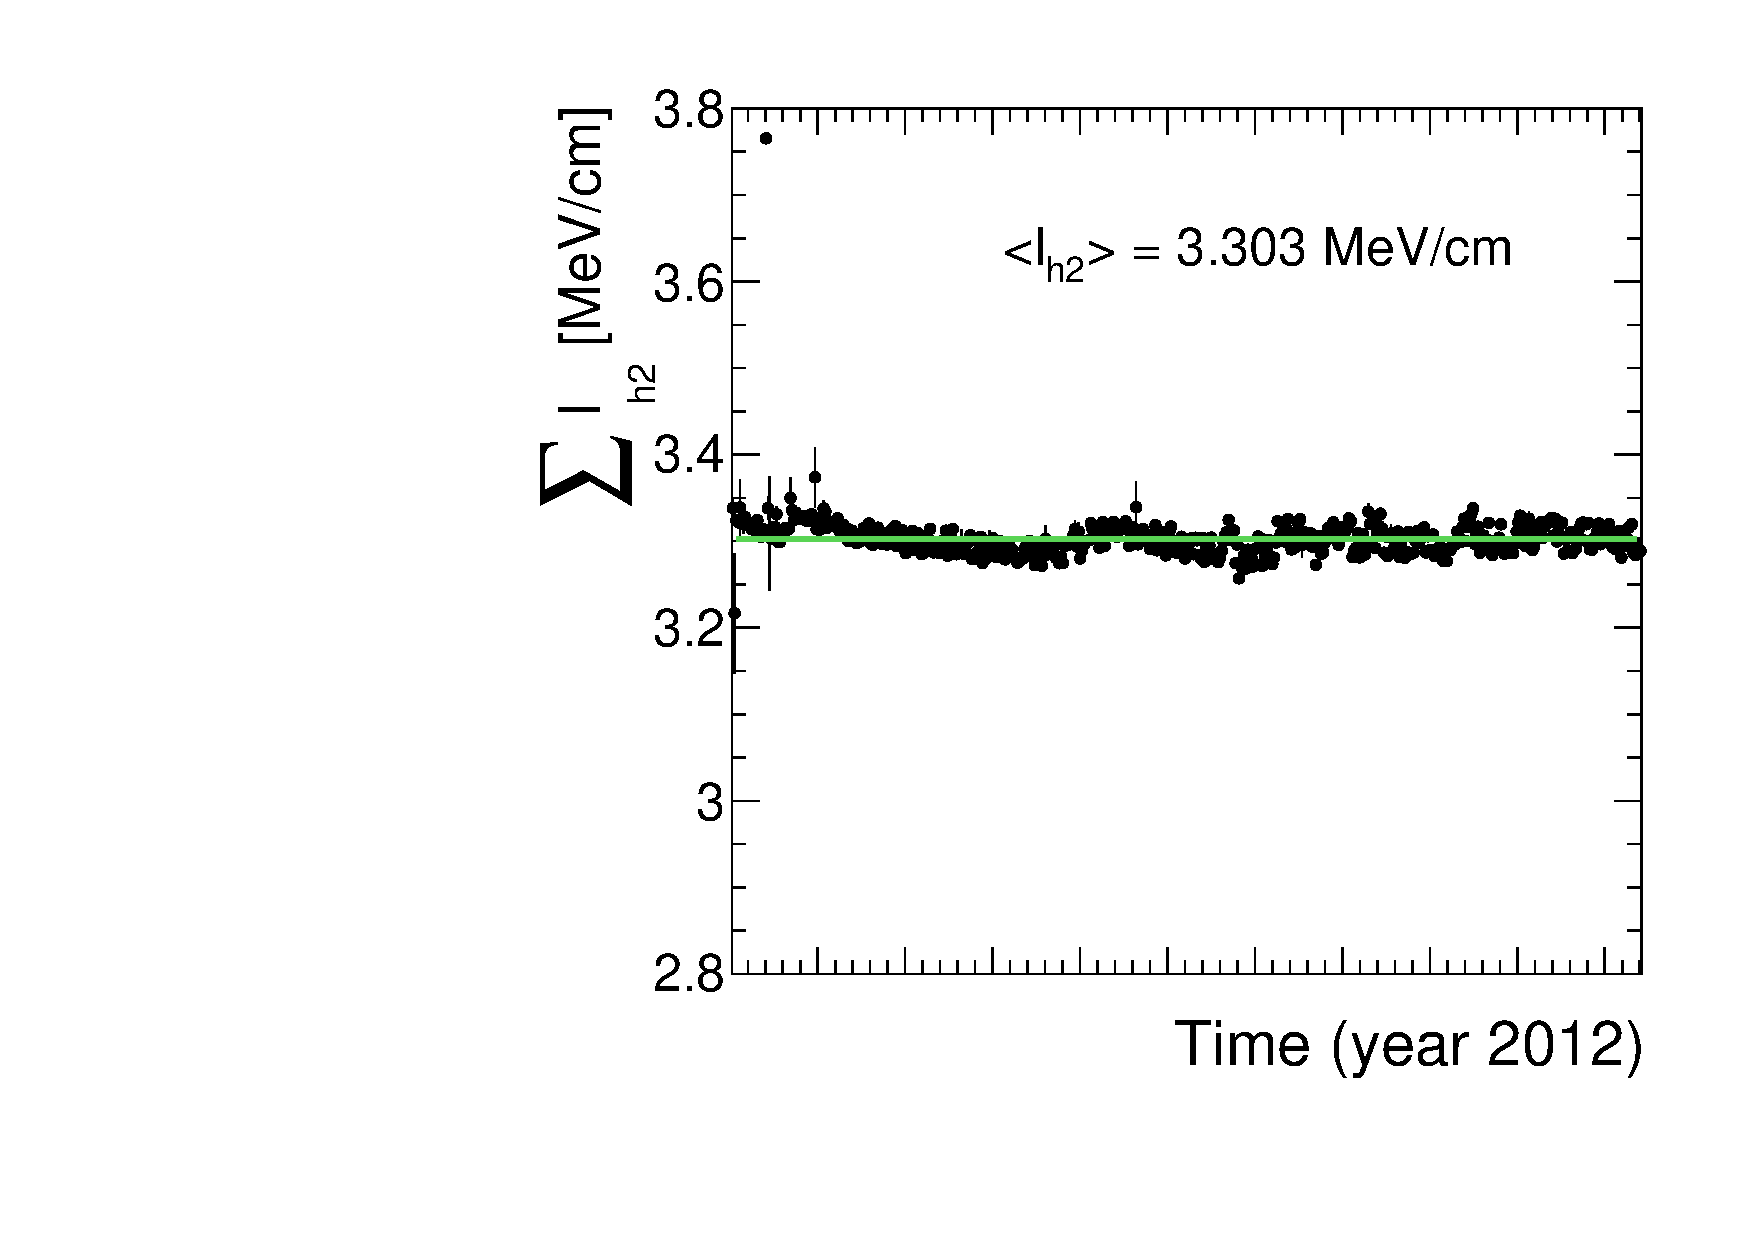
\includegraphics[width=0.49\textwidth]{figures/analysis/PixelCalibration/StabilityPlot_Strip_afterCalibration_withoutStepFits_NEW.pdf}
  \end{tabular}
  \caption{Sum of all track's $dE/dx$ (harmonic-2 estimator) measured in the silicon strip detector over the full year 2012. The average most probable $dE/dx$ is $\ihtwo=3.303\,\mev/\cm$. Every data point corresponds to one run.} 
  \label{fig:StabilityPlot_Strip}
\end{figure}
This factor is then applied on top of $c_{\text{inter}}$ for all pixel modules.

Finally, an absolute calibration factor needs to be determined for the simulated samples, where the simulated pixel tracker is calibrated to the average $dE/dx$ of the silicon strip measured in data.

\section{Discrimination of highly-ionising particles}

As mentioned before, it is difficult to find a robust estimator for the MPV of the Landau distribution, if only a few single measurements of $\Delta E/ \Delta x$  are available.
The harmonic-2 estimator \ihtwo was already introduced in Section~\ref{sec:sub:MeasuringDeDx} in Eq.~\ref{eq:Harmonic2Estimator}.
It is known to be a robust estimator not easily biased by large fluctuation in $\Delta E/ \Delta x$ because of the suppression by a factor of two.

However, it was shown in \cite{bib:Quertenmont_2010} that a better discrimination between SM particles and possible new heavy particles can be achieved when using likelihood techniques,
i.e. determining the probability that the set of all $\Delta E/ \Delta x$ belonging to one track is actually compatible with the hypothetical probability distribution of a MIP.

Testing that a measured sample has been drawn from a specific distribution is known as the Smirnov-Cram\'{e}r-von Mises test \cite{bib:Anderson:CramerVonMises_1962,bib:James:StaticticalMethods_2006},
which is deduced from the integral of the squared difference of the measured distribution $P_N(x)$ to the hypothesis distribution $P(x)$
\begin{equation*}
I_s = \int\limits_{-\infty}^{\infty} \left[P_{N}(x)-P(x)\right]^2 dP(x)
\end{equation*}
leading to a test statistics of
\begin{equation*}
I_s = \frac{3}{N} \cdot \left( \frac{1}{12N} + \sum\limits_{i=1}^N \left[ P_i - \frac{2i-1}{2N} \right]^2 \right),
\end{equation*}
where N is the total number of energy measurements and $P_i$ is the cumulative probability that a MIP would release a $\Delta E/\Delta x$ equal or smaller than the measured $\Delta E/ \Delta x$ with all $P_i$ are arranged in increasing order.

However, this test statistics is not sensitive to the sign of the difference between the measured and the theoretical distribution.
It can therefore not distinguish between incompatibilities due to variations towards higher or lower energy deposits compared to the hypothesis distribution.
Thus it is not suitable for the discrimination between MIPs and heavy new particles by $dE/dx$.
A so-called Asymmetric Smirnov-Cram\'{e}r-von Mises discriminator was developed in \cite{bib:Quertenmont_2010} which is only sensitive to incompatibilities to the MIP hypothesis towards higher energy depositions
\begin{equation*}
\ias = \frac{3}{N} \cdot \left( \frac{1}{12N} + \sum\limits_{i=1}^N \left[ P_i \cdot \left(P_i - \frac{2i-1}{2N} \right)^2 \right] \right).
\end{equation*}
A value of \ias close to zero indicates good compatibility with the MIP hypothesis, whereas a value close to one indicates worse compatibility because of unexpectedly high energy losses.

The underlying probability P$_i$ of the energy release for a given path length in the pixel tracker is extracted from the same ``Minimum bias'' sample used for the pixel energy calibration.
In total 28 different templates each for a different given path length are created.
In Fig.~\ref{fig:ProbabilityTemplate} the probability distribution template for the pixel tracker in data and simulation is shown.
The corresponding templates for the energy release in the silicon strip detector were already built by  \cite{bib:Quertenmont_2010}.


A comparison between the energy release by MIPs (\ias) in data and simulation for good quality tracks with $p>5\gev$ and $|\eta|<2.1$ can be found in Fig.~\ref{fig:Data-MC-Dedx_MIPs}.
\begin{figure}[!tb]
  \centering 
  \begin{tabular}{c}
    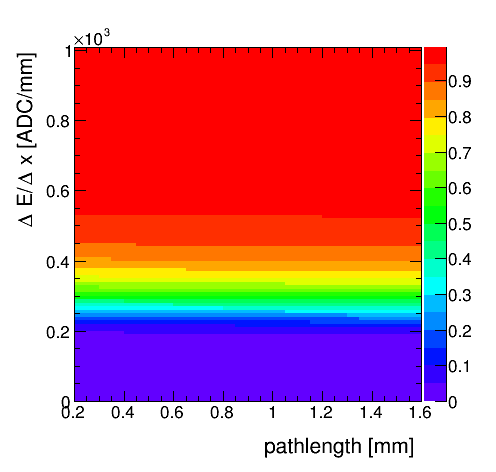
\includegraphics[width=0.49\textwidth]{figures/analysis/Discriminator_template_data_pixel_2012.png}
    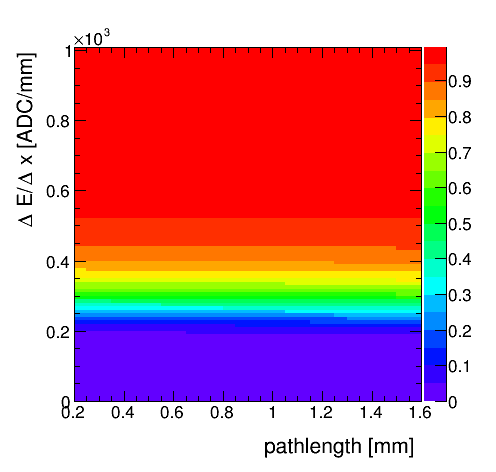
\includegraphics[width=0.49\textwidth]{figures/analysis/Discriminator_template_mc_pixel_2012.png}
  \end{tabular}
  \caption{Cumulative probability for a MIP to release a $\Delta E/ \Delta x$ (y-axis) vs. the path length (x-axis) in data (left) and simulation (right) for the pixel tracker based on the ``Minimum bias'' sample.}
  \vspace{60pt}
  \label{fig:ProbabilityTemplate}
\end{figure}
\begin{figure}[!bt]
  \centering 
  \begin{tabular}{c}
    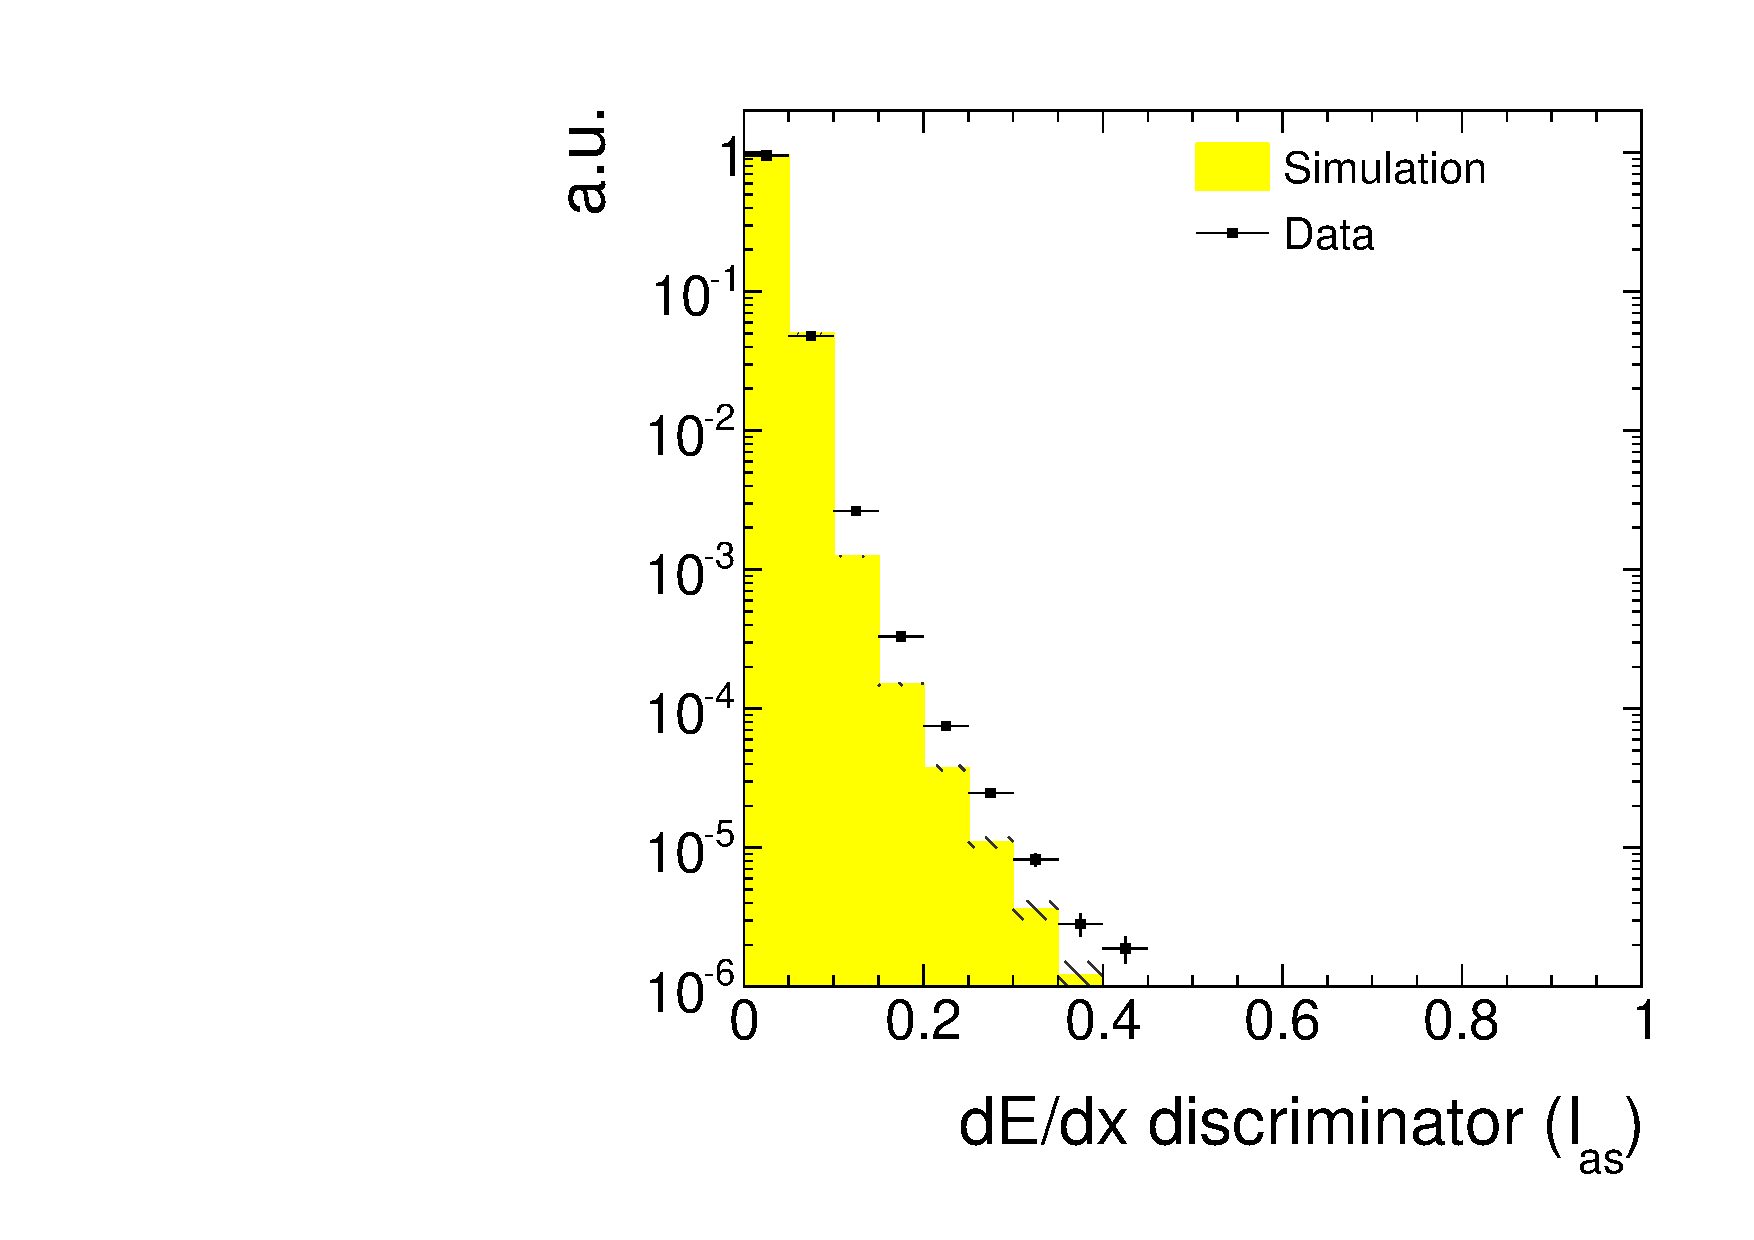
\includegraphics[width=0.49\textwidth]{figures/analysis/PixelCalibration/htrackASmiSmallRange_log_MIPs.pdf}
  \end{tabular}
  \caption{Normalised \ias distribution for MIPs from the minimum bias sample in data and simulation for good quality (high-purity as defined in \cite{bib:CMS:Tracking_2010} and minimum number of eight hits) tracks with $p>5\gev$ and $|\eta|<2.1$.}
  \label{fig:Data-MC-Dedx_MIPs}
\end{figure}
$dE/dx$ shows good agreement in data and simulation for $\ias<0.1$.
For larger values, \ias shows a larger decrease in simulation than in measured data.
That's the reason why a data-based approach for analyses exploiting $dE/dx$ information is needed.\\

\newpage
\section{Discrimination improvements}
The goal of including the pixel energy information is to increase the discrimination power of \ias between background and signal tracks, especially for shorter lifetimes.
In Fig.~\ref{fig:MIPs-Signal-Dedx}, a comparison of the shapes of the energy release by MIPs and by signal tracks in simulation is shown (details about the simulated samples can be found in the next section Section~\ref{sec:SignalSamples}).
\begin{figure}[!b]
  \centering 
  \begin{tabular}{c}
    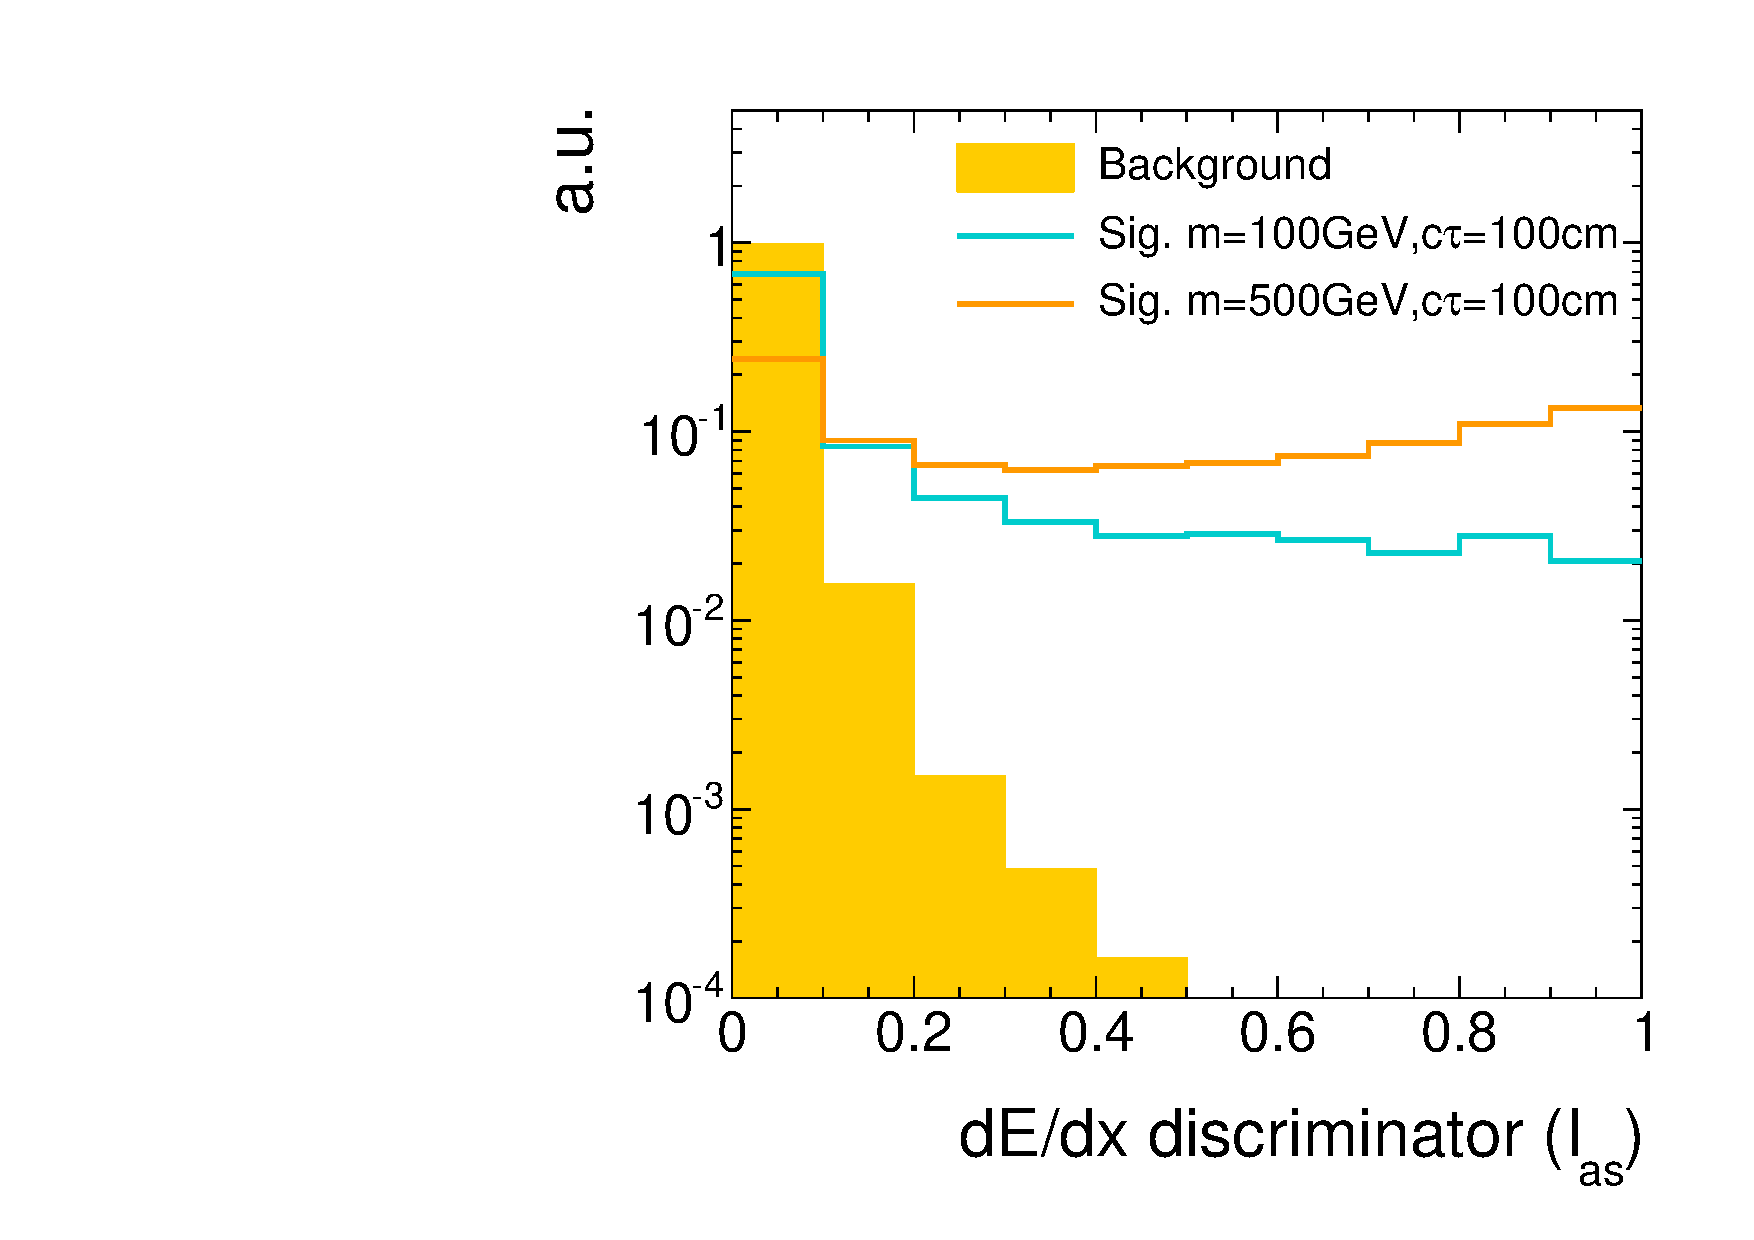
\includegraphics[width=0.49\textwidth]{figures/analysis/PixelCalibration/htrackASmiSmallRange_log_chiTracksGoodQualitySelection_2Signal_ttjets.pdf}   
    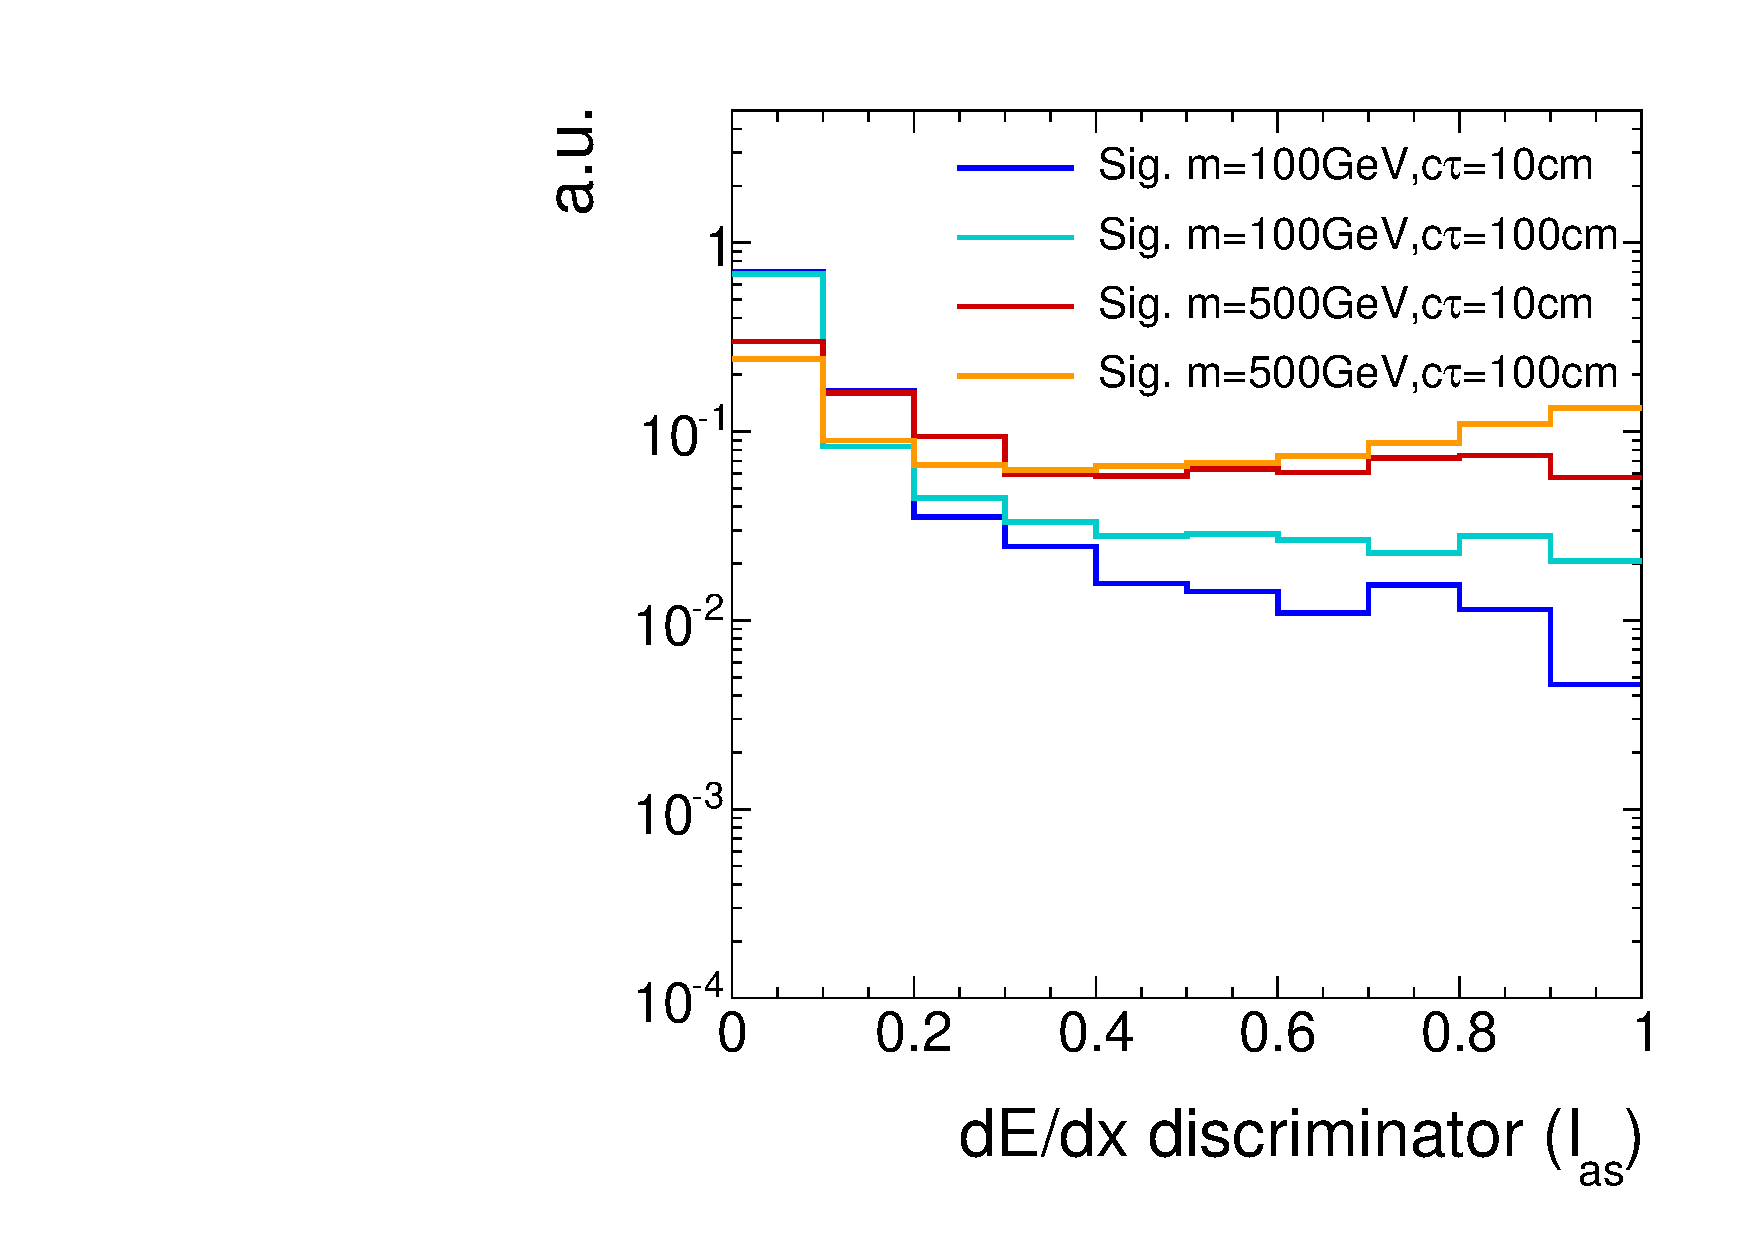
\includegraphics[width=0.49\textwidth]{figures/analysis/PixelCalibration/htrackASmiSmallRange_log_chiTracksGoodQualitySelection_4Signal.pdf}
  \end{tabular}
  \caption{Normalised \ias distribution for simulated background and signal tracks (left) and for four different signal models (right) 
           for high-purity tracks (as defined in \cite{bib:CMS:Tracking_2010}) with \pt$>10\gev$ and $|\eta|<2.1$.
           For the illustration of the background tracks' spectrum simulated $t\bar{t}$+jets events are used (more information about this sample is given in Section~\ref{sec:SimulatedSamples}).}
  \label{fig:MIPs-Signal-Dedx}
\end{figure} 
It can be seen, that the \ias distributions of all signal models show a larger tail towards $\ias=1$, whereas the \ias of the background is rapidly falling.
The \ias distribution is not only influenced by the velocity ($\beta$) of a particle but also by the number of hits of a track.
The influence of the velocity can be easily seen in Eq.~\ref{eq:Landau_Vavilov_Bichsel}. 
This in turn results in a dependency of \ias on the mass of the incident particle.
However, also for charginos with same mass, the velocity is higher in average for shorter lifetimes.
This is caused by the fact, that for shorter lifetimes (e.g. $\ctau=10\cm$), already a sizable fraction of the charginos decay before reaching the tracker system.
The probability of reaching the detector increases for higher velocities because of the boost, which can be clearly seen at the survival probability
\begin{equation}
P \left( t \right) = e^{-\frac{t}{\gamma \tau}}.
\end{equation} 
This means that shorter lifetimes lead to higher average $\beta$ which in turn lead to lower values of \ias.

The number of measurements in the tracker system defines the influence of single fluctuations in $\Delta E/\Delta x$ on the \ias discriminator, because of the long right tail of the Landau distribution, A low number of hits lead therefore to higher \ias values.

Thus, \ias for charginos with lower lifetimes are affected by two things: 
First, due to the smaller number of measurements the chargino tends to higher \ias values.
Second, low lifetimes charginos have in average a higher velocity leading to lower \ias values.
Both effects can be seen in Fig.~\ref{fig:MIPs-Signal-Dedx} (right).
The large tail for longer lifetimes is caused by the lower velocities, but the small surplus between 0.1 and 0.2 is caused by the smaller number of measurements for lower lifetimes.\\


Finally, the impact of the additional $\Delta E/\Delta x$ information from the pixel tracker on the selection efficiency of signal and background tracks is quantified.
Figure~\ref{fig:ROCplots} shows the signal selection efficiency against the background selection efficiency for different selection cuts in \ias, once including the pixel information and once without it.
The background selection efficiency is estimated with simulated $W$+jets  events but was additionally checked on simulated $t\bar{t}$+jets  and QCD-multijet events 
(further information about the simulated samples can be found in the next section).
No significant difference between these processes in the background selection efficiency was observed.

The signal selection efficiency and the background suppression depend on the mass and the lifetime of the charginos.
The discrimination power of \ias is much better for higher masses as expected.

It can be seen that the inclusion of the pixel information increases the background suppression for a given signal efficiency throughout the investigated signal models.
This background suppression improvement is most pronounced for very tight cuts on \ias (up to a factor of 20) and still considerable for looser selections with signal efficiencies of around 40\% (factor of 10).

\begin{figure}[!bt]
  \centering 
  \vspace{79pt}
  \begin{tabular}{c}
    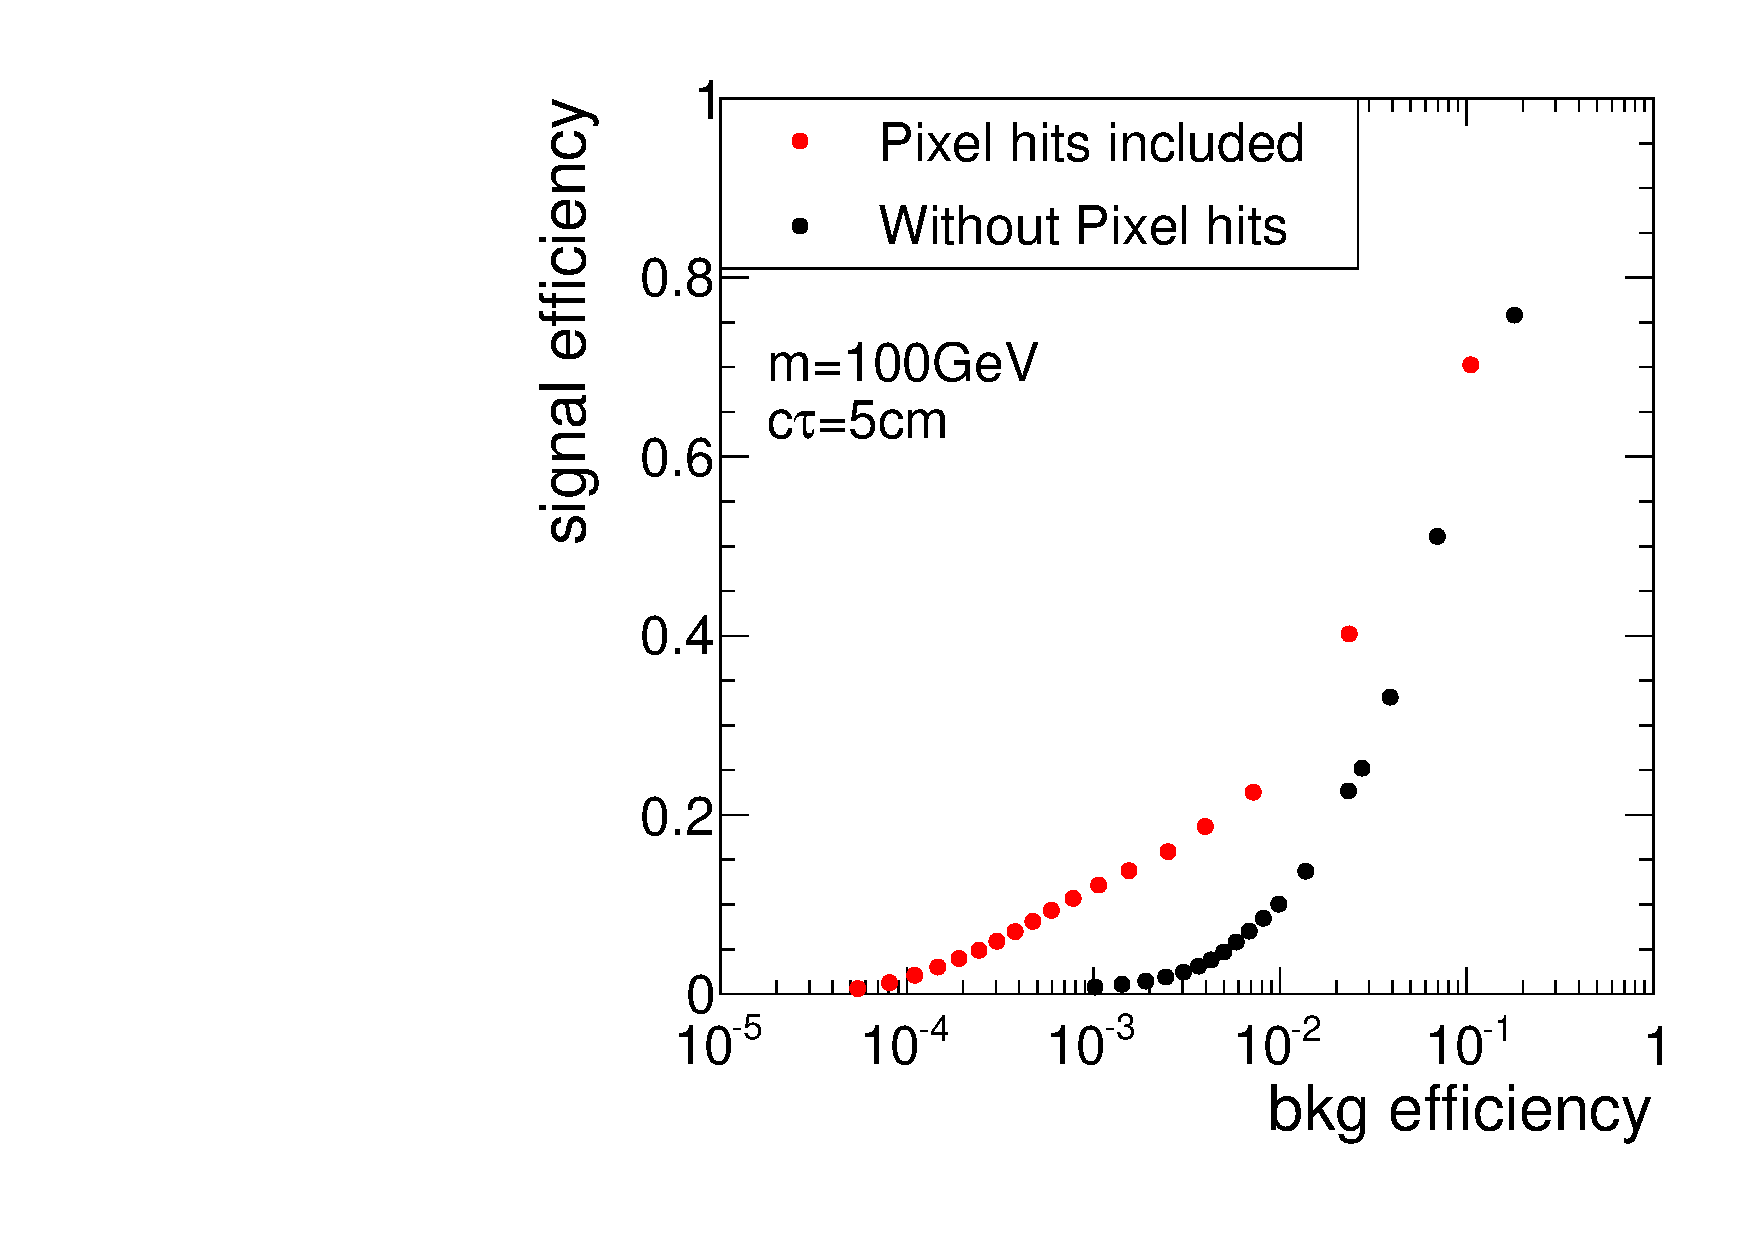
\includegraphics[width=0.49\textwidth]{figures/analysis/rocplot_wjets_mass_100GeV_ctau_5cm.pdf} 
    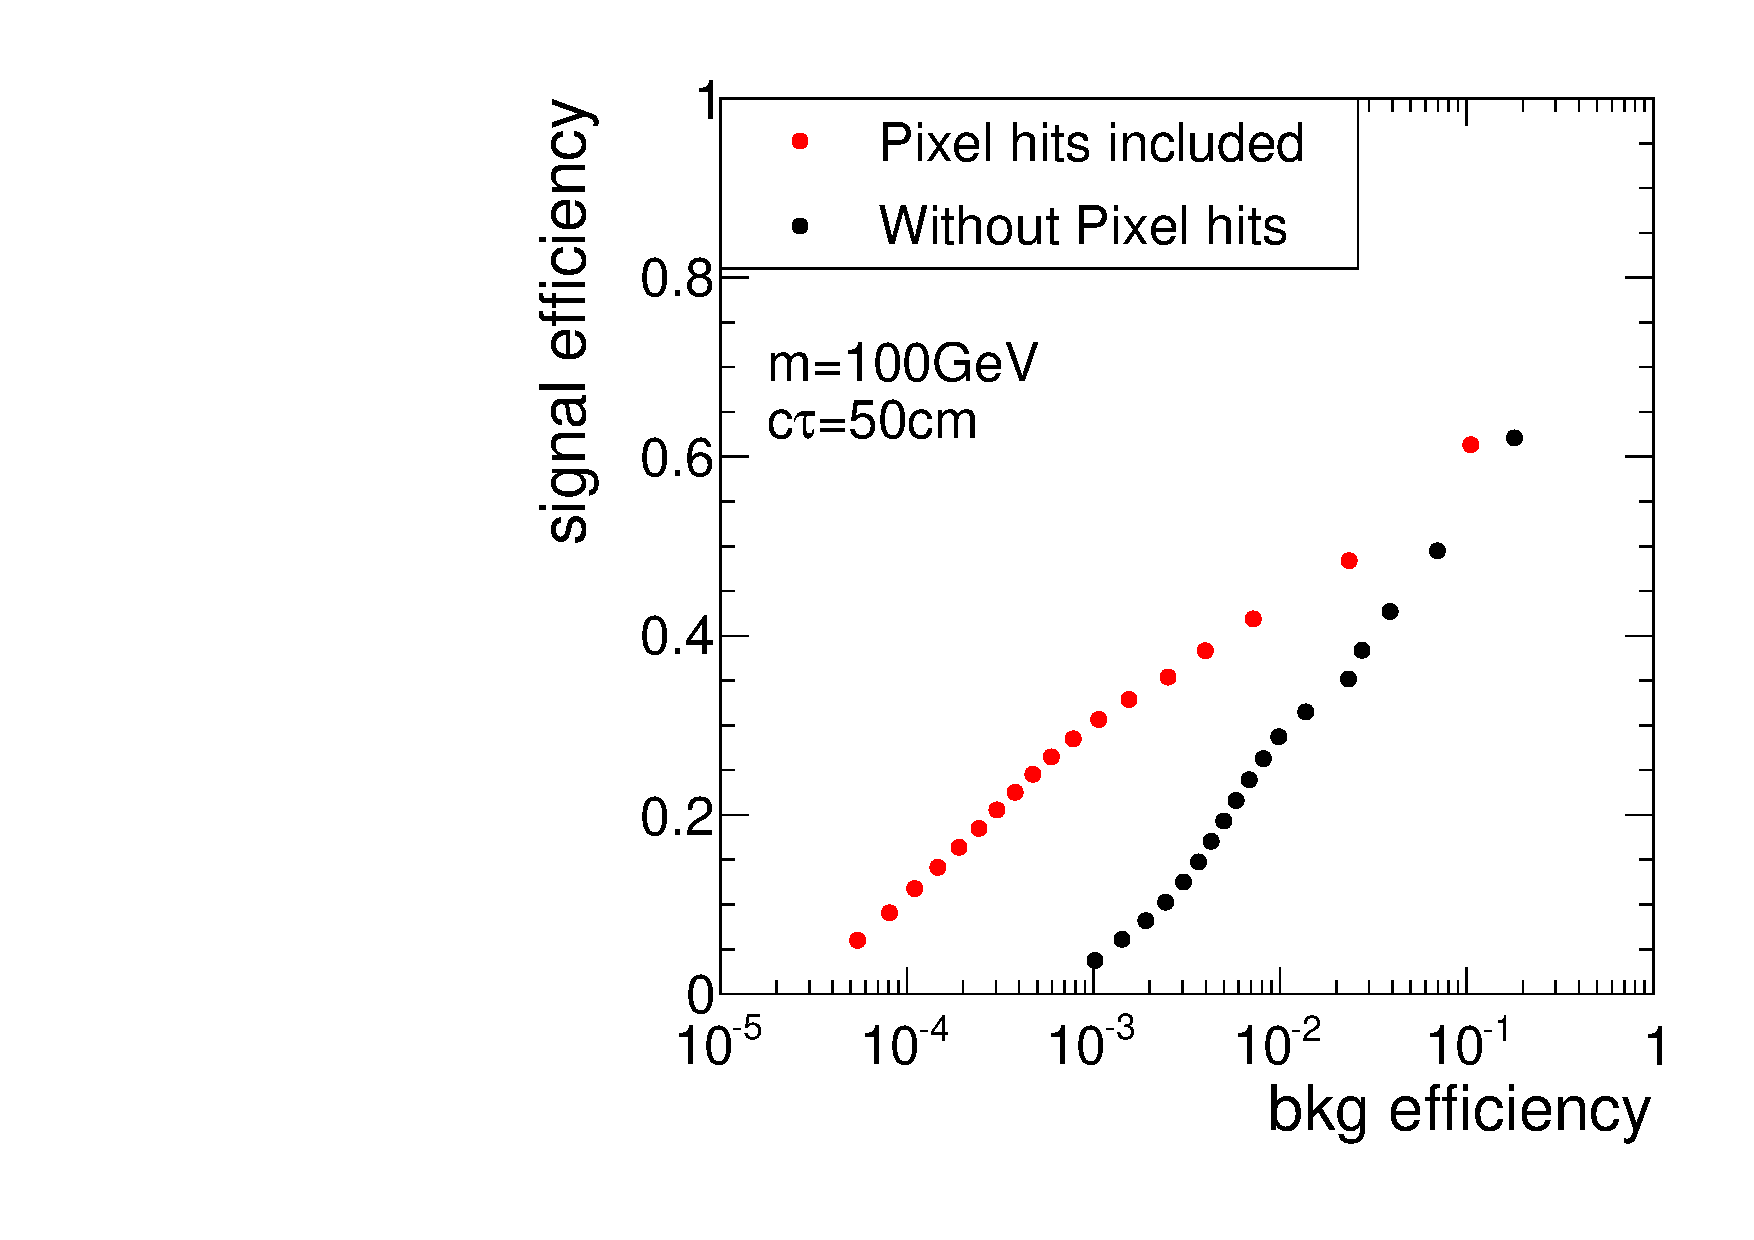
\includegraphics[width=0.49\textwidth]{figures/analysis/rocplot_wjets_mass_100GeV_ctau_50cm.pdf} \\
    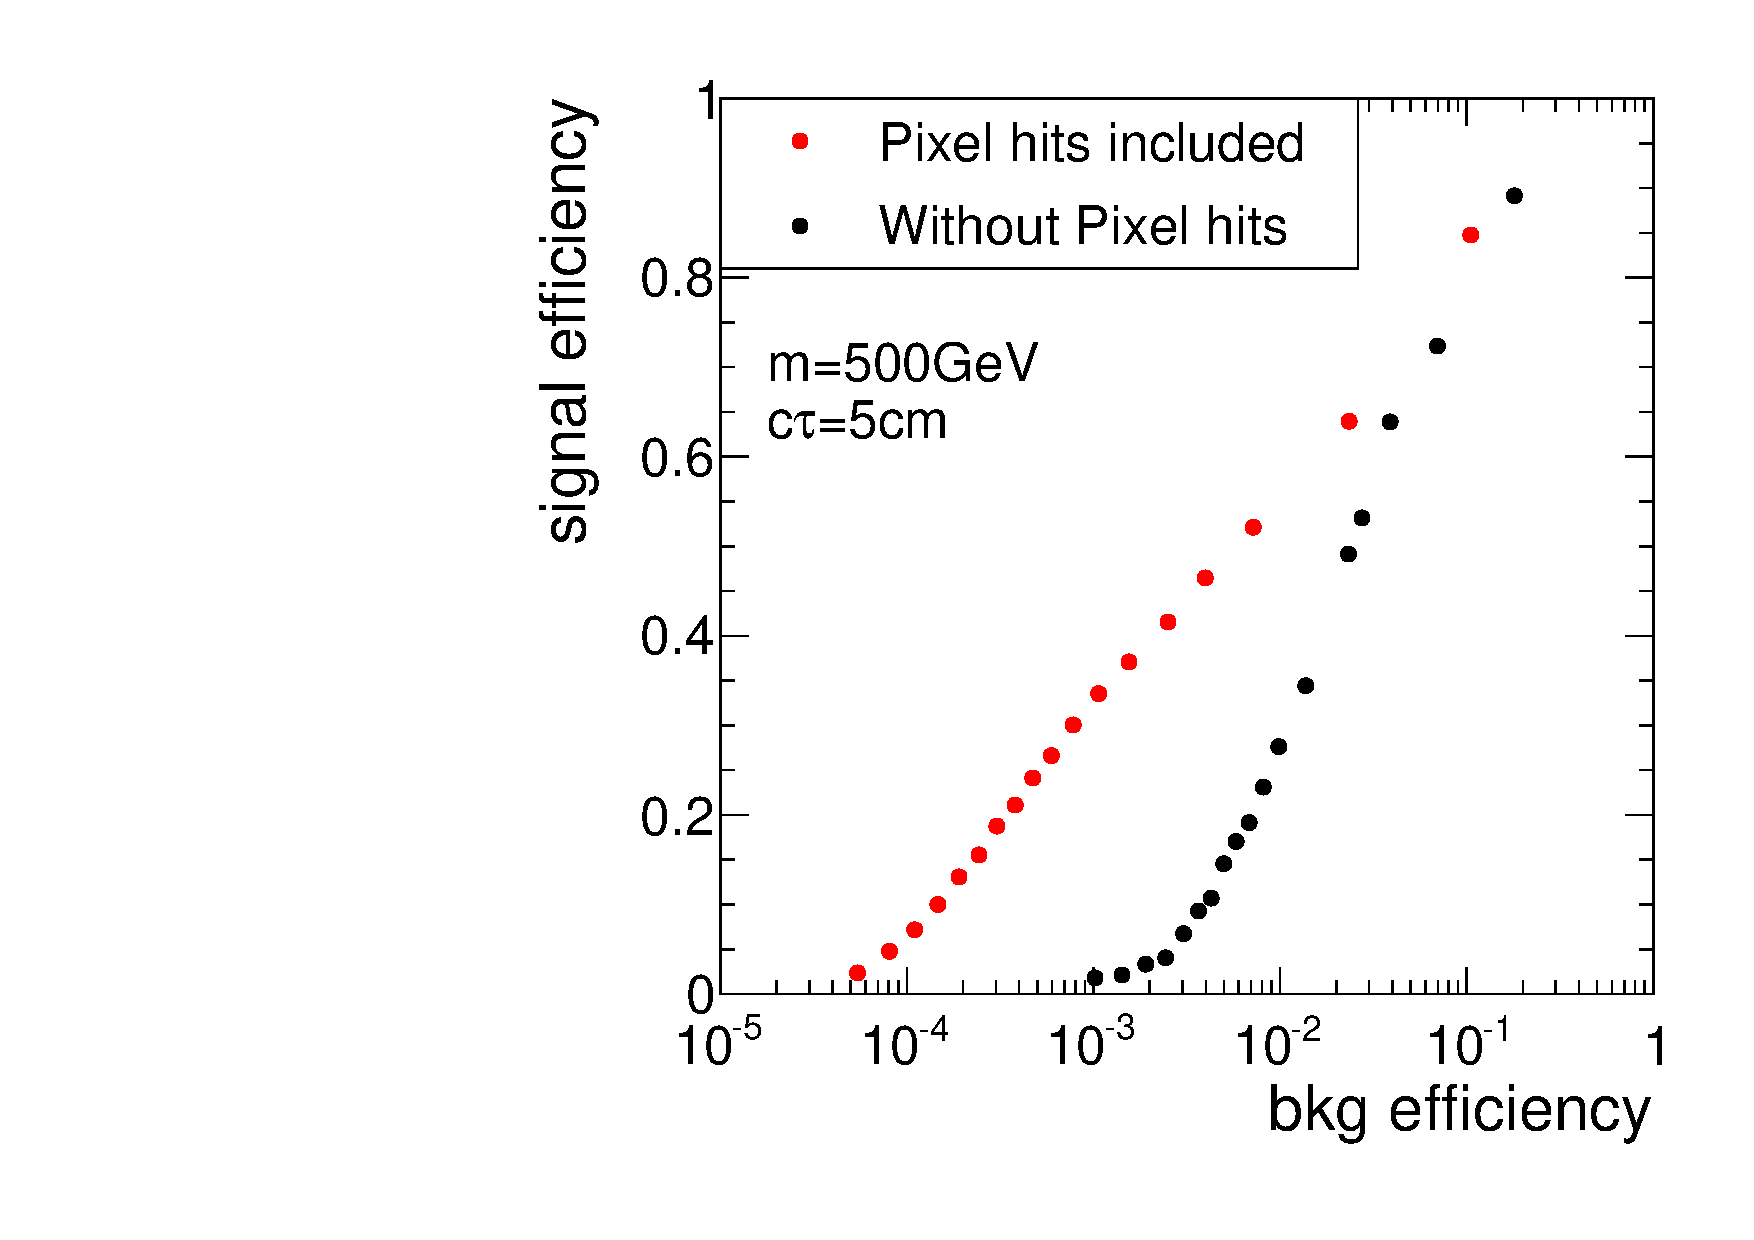
\includegraphics[width=0.49\textwidth]{figures/analysis/rocplot_wjets_mass_500GeV_ctau_5cm.pdf} 
    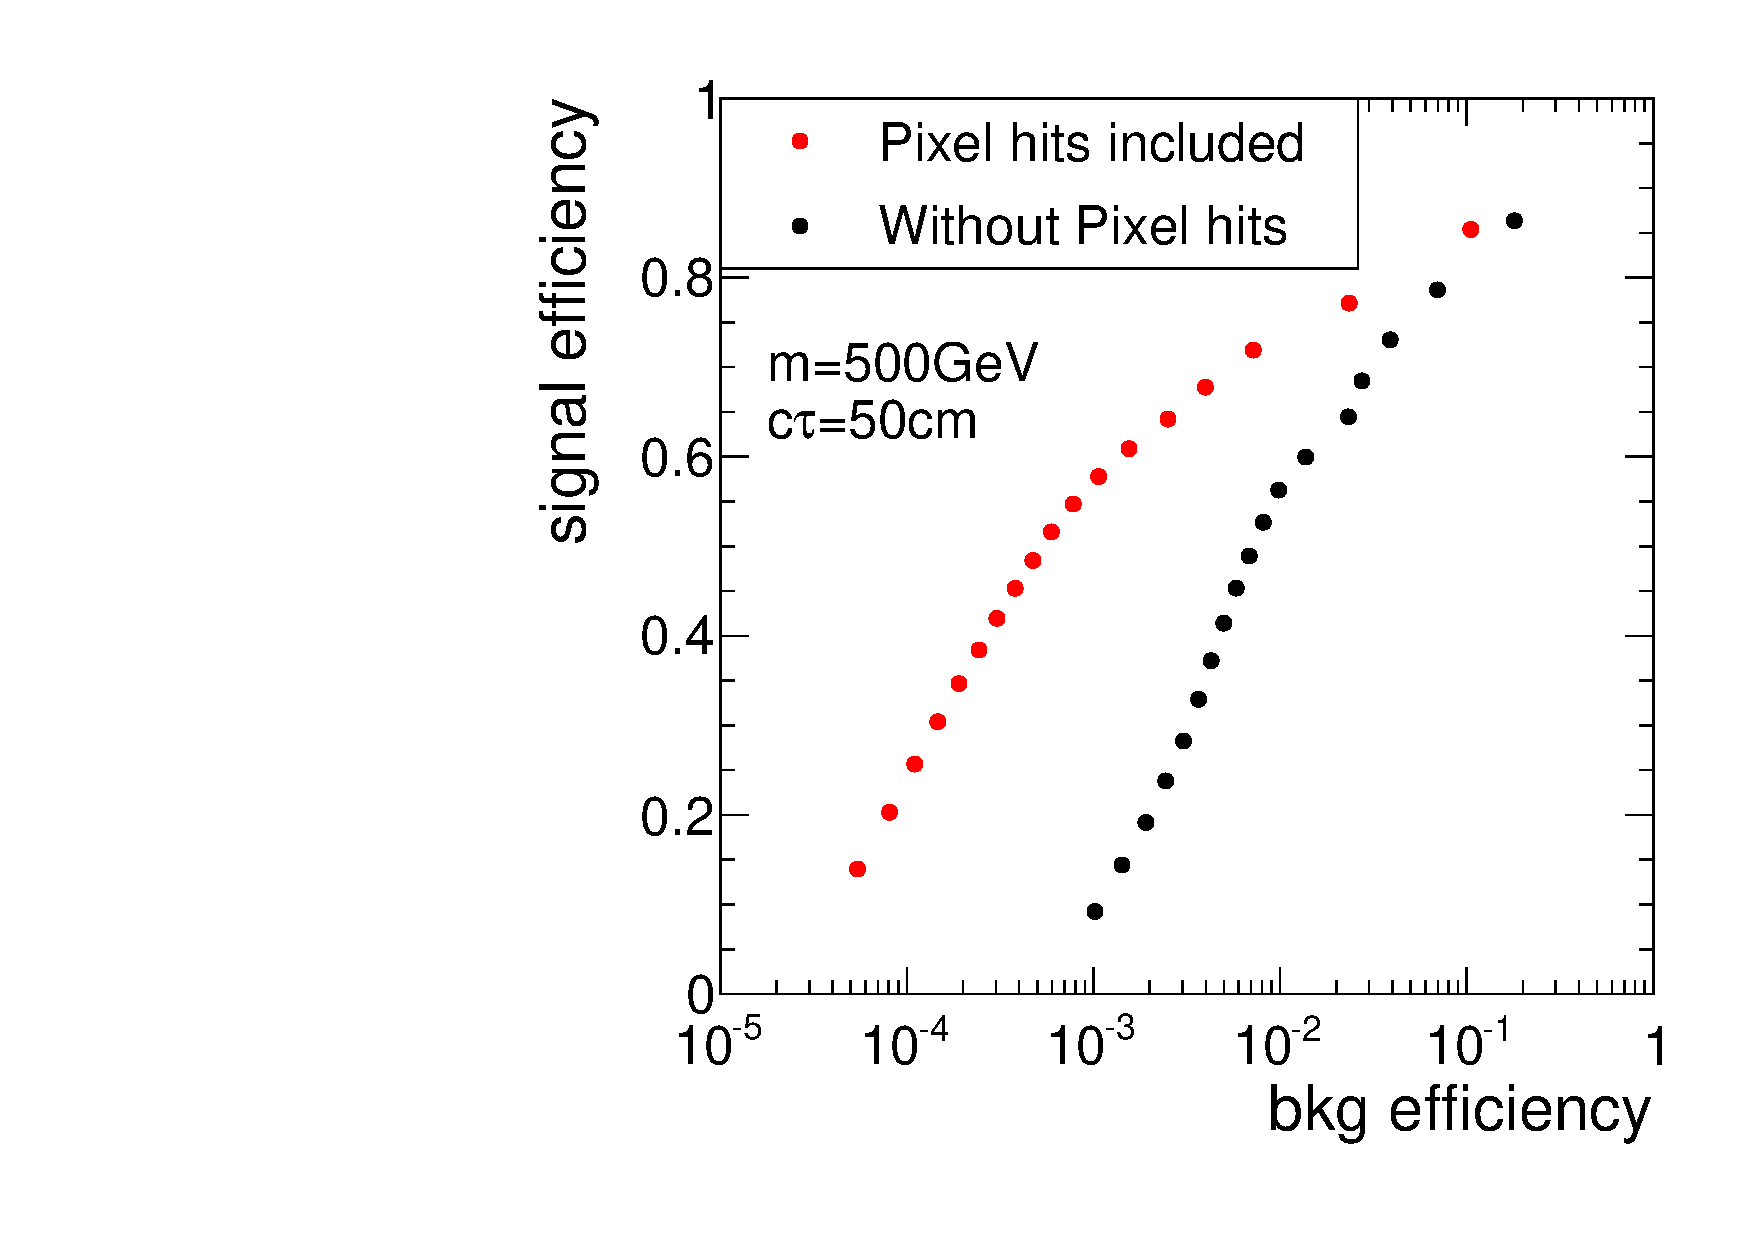
\includegraphics[width=0.49\textwidth]{figures/analysis/rocplot_wjets_mass_500GeV_ctau_50cm.pdf}
  \end{tabular}
  \caption{Signal selection efficiency vs. background selection efficiency with (red) and without (black) pixel information.
           Each point correspond to one selection cut in \ias.
           The figure is based on a simulated \WJets sample and a simulated signal sample with chargino-chargino production, both subject to a selection of good quality tracks with $\pt>10\gev$.
       }
  %\vspace{40pt}
  \label{fig:ROCplots}
\end{figure} 
%%%%%%%%%%%%%%%%%%%%%%%%%%%%%%%%%%%%%%%%%%%%%%%%%%%%%%%%%%%%%%%%%%%%%%%%%%%%%%%%%%%%%%%%%%%%%%%%%%%%%%%%%%%%%%%%%%%%%%%%%%%%%%%%%%%%%%%%%%%%%%%%%%%%%%%%%%%%%%%%%%%%%%%%%%%%%%%%%%%%
%%%%%%%%%%%%%%%%%%%%%%%%%%%%%%%%%%%%%%%%%%%%%%%%%%%%%%%%%%%%%%%%%%%%%%%%%%%%%%%%%%%%%%%%%%%%%%%%%%%%%%%%%%%%%%%%%%%%%%%%%%%%%%%%%%%%%%%%%%%%%%%%%%%%%%%%%%%%%%%%%%%%%%%%%%%%%%%%%%%%
